%% TeX Preamble
\documentclass[12pt,twoside]{reedthesis}
%=================
%     PACKAGES
%=================
\usepackage{graphicx,latexsym}
\usepackage{amssymb,amsthm,amsmath}
\usepackage{physics}
\usepackage{longtable,booktabs,setspace}
\usepackage{euscript}
\usepackage{dsfont} % Boldface 1 for indicator function
\usepackage{array} % For the analytical eigenvector proof (block matrices)


%==================
%     COMMANDS
%==================
% Latin Letters (bb)
\newcommand{\Cc}{\mathbb{C}} % Complex Numbers
\newcommand{\R}{\mathbb{R}} % Reals
\newcommand{\N}{\mathbb{N}} % Naturals
\newcommand{\F}{\mathbb{F}} % Field

% Latin Letters (cal)
\newcommand{\B}{\mathcal{B}} % Batch
\newcommand{\Rseq}{\mathcal{R}} % Ratio-Sequence
\newcommand{\Seq}{\mathcal{S}} % Sequence
\renewcommand{\S}{\mathbb{S}} % Spectrum
\newcommand{\Ens}{\mathcal{E}} % Ensemble
\newcommand{\D}{\mathcal{D}} % Distribution

% Greek letters
\renewcommand{\epsilon}{\varepsilon}
\newcommand{\ep}{\epsilon}
\renewcommand{\d}{\delta}
\renewcommand{\b}{\beta}

% Probability & Probability Distributions
\newcommand{\Prb}{\text{P}}
\newcommand{\E}{\mathbb{E}}
\newcommand{\Var}{\text{Var}}
\newcommand{\Unif}{\text{Unif}}
\newcommand{\Bern}{\text{Bern}}
\newcommand{\Bin}{\text{Bin}}
\newcommand{\Normal}{\mathcal{N}}

% Math macros
\newcommand{\oneto}[1][n]{1,\dots,#1} % 1,...,n
\newcommand{\sumi}[1][n]{\sum_{i = 1}^{#1}} % sum from i = 1 to n
\newcommand{\seq}[2][n]{{{#2}_0,{#2}_1,\dots,{#2}_{#1}}} % x_1,...,x_n

% Words
\newcommand{\where}{\text{ where }}
\newcommand{\for}{\text{ for }}
\newcommand{\given}{\text{ given }}
\renewcommand{\and}{\text{ and }}

% Other
\newcommand{\ra}{\rightarrow}

%==================
%     SLIDES
%==================

%========================
%     SLIDE SECTIONS
%========================
\AtBeginSection[]{
  \begin{frame}
  \vfill
  \centering
  \begin{beamercolorbox}[sep=8pt,center,shadow=true,rounded=true]{title}
    \usebeamerfont{title}\insertsectionhead\par%
  \end{beamercolorbox}
  \vfill
  \end{frame}
}

%=====================
%     SLIDE TITLES
%=====================
\newcommand{\deftitle}[1]{\textbf{Definition:}$\;$#1}
\newcommand{\thmtitle}[1]{\textbf{Theorem:}$\;$#1}
\newcommand{\remtitle}[1]{\textbf{Remark:}$\;$#1}


%==================
%     TABLES
%==================
%============================
%      D-DISTRIBUTIONS
%============================
\newcommand{\Ddisttable}{
  \begin{tabular}{ |p{3cm}||p{3cm}|p{3cm}|p{3cm}|  }
   \hline
   \multicolumn{4}{|c|}{Table of Random Matrix Distributions} \\
   \hline
   Distribution & Notation ($\D$) & Parameters & Class\\
   \hline
   Normal & $\Normal(\mu,\sigma)$ & $\mu \in \R, \sigma \in \R^+$  &  Explicit\\
   Uniform  & $\Unif(a,b)$ & $a,b \in \R$ & Explicit\\
   Hermite-$\beta$   & $\mathcal{H}(\beta)$  &  $\b \in \N$  & Implicit\\
   Erdos-$p$   &   $\text{ER}(p)$  & $p \in [0,1]$   & Implicit\\
   \hline
  \end{tabular}
}
%============================
%      SPECTRUM SCHEMES
%============================
\newcommand{\spectrumschemetable}{
  \begin{tabular}{ |p{3cm}||p{2cm}|p{2.5cm}|p{4.5cm}|  }
   \hline
   \multicolumn{4}{|c|}{Table of Spectrum Schema} \\
   \hline
   Scheme & Matrix & Notation & Ordering \\
   \hline
   Sign-Ordered & $P$ & $\sigma_{S}(P)$ & $\lambda_1 \geq \lambda_2 \geq ... \geq \lambda_N$ \\
   Norm-Ordered & $P$ & $\sigma_{N}(P)$ & $|\lambda_1| \geq |\lambda_2| \geq ... \geq |\lambda_N|$ \\
   Singular & $P \cdot P^T$ & $\sigma_{+}(P)$ & $\sqrt{\lambda_1} \geq \sqrt{\lambda_2} \geq ... \geq \sqrt{\lambda_N}$ \\
   \hline
  \end{tabular}
}
%============================
%     DISPERSION METRICS
%============================
\newcommand{\dispersiontable}{
  %\begin{tabular}{ |p{5cm}||p{2cm}|p{2cm}|p{2cm}|p{2cm}|  }
  \begin{tabular}{ |p{4.4cm}||p{1.9cm}|p{1.9cm}|p{1.9cm}|p{1.9cm}|  }
   \hline
   \multicolumn{5}{|c|}{Table of Dispersion Metrics} \\
   \hline
   Metric* & Notation & Formula & Symmetric & Parameters\\
   \hline
   Standard Norm & $\d$ & $|z' - z|$ &  True & - \\
   $\beta$-Norm & $\d_\b$ & $|z' - z|^\b$ & True & $\b \in \N$ \\
   Difference of Absolutes & $\d_{\text{abs}}$ & $|z'| - |z|$ &  False  &  - \\
   Identity Difference &  $\d_{\text{id}}$ & $z' - z$ & False &  - \\
   %Angola & AO & AGO & 024\\
   \hline
  \end{tabular}
}
%============================
%      PAIRING SCHEMES
%============================
\newcommand{\pairingschemetable}{
  %\begin{tabular}{ |p{2.5cm}||p{1.75cm}|p{5.5cm}|  }
  %\begin{center}
    \begin{tabular}{ |p{3cm}||p{3cm}|p{6cm}|  }
     \hline
     \multicolumn{3}{|c|}{Table of Pairing Schema} \\
     \hline
     Scheme & Notation & Formula \\
     \hline
     Lower & $\Pi_<$ & $\{(i,j) \mid i < j \for i,j \in \N_N \}$ \\
     Upper  & $\Pi_>$ & $\{(i,j) \mid i > j \for i,j \in \N_N \}$ \\
     Consecutive  & $\Pi_C$ & $\{(i,j) \mid i = j + 1 \for i,j \in \N_N \}$ \\
     All & $\Pi_0$ & $\{(i,j) \mid i,j \in \N_N \}$ \\
     \hline
    \end{tabular}
  %\end{center}
}


%==================
%     GRAPHICS
%==================
%==================
%     CHAPTER 2
%==================

\newcommand{\FIGUREspectrumcomparison}[2]{
  \begin{figure}[#1]
   \begin{center}
    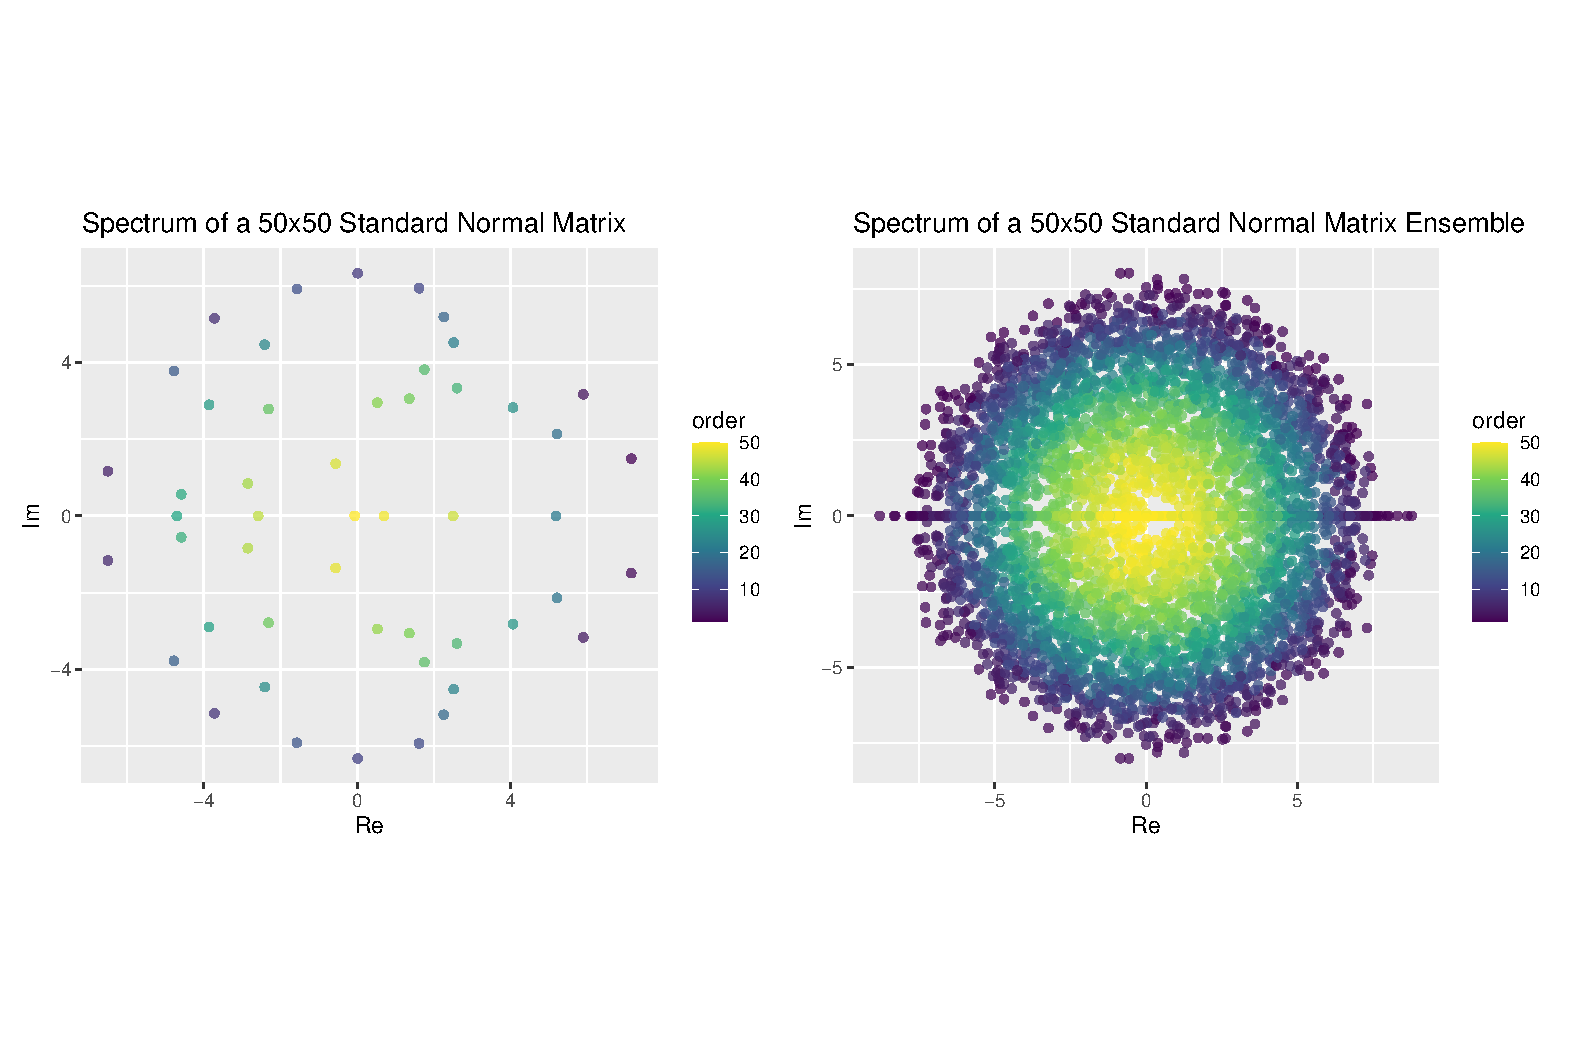
\includegraphics[scale = #2]{../graphics/chap2/2-1-2_comparison}
    \caption{Spectrum of a Matrix versus an Ensemble}
   \end{center}
   \label{ensemble_comparison_plot}
  \end{figure}
}

\newcommand{\FIGUREnormalspectrum}[2]{
  \begin{figure}[#1]
   \begin{center}
    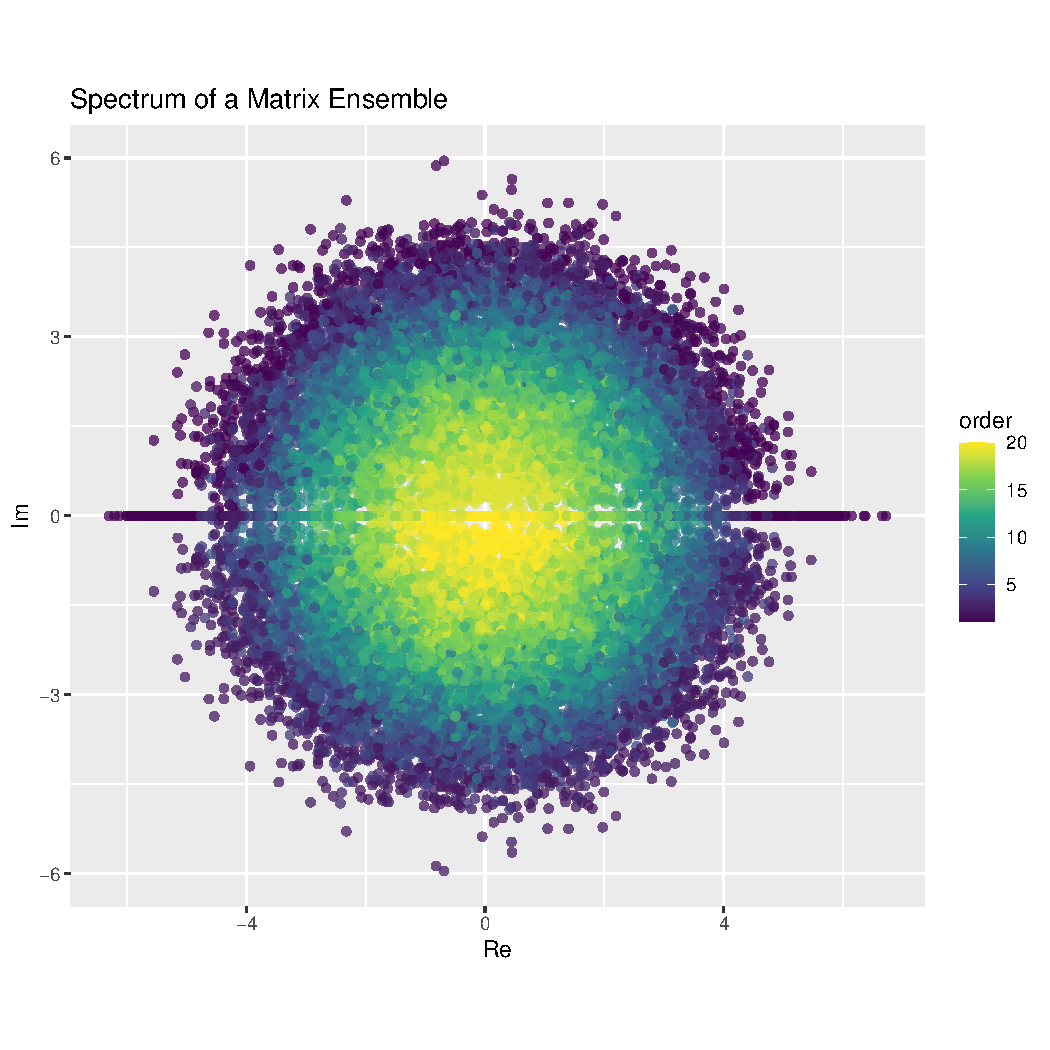
\includegraphics[scale = #2]{../graphics/chap2/2-1-2_normal_spec}
    \caption{Spectrum of a Standard Normal Matrix ensemble}
   \end{center}
   \label{spectrum_normal_ensemble_plot}
  \end{figure}
}

\newcommand{\FIGUREorderscheme}[2]{
  \begin{figure}[#1]
   \begin{center}
    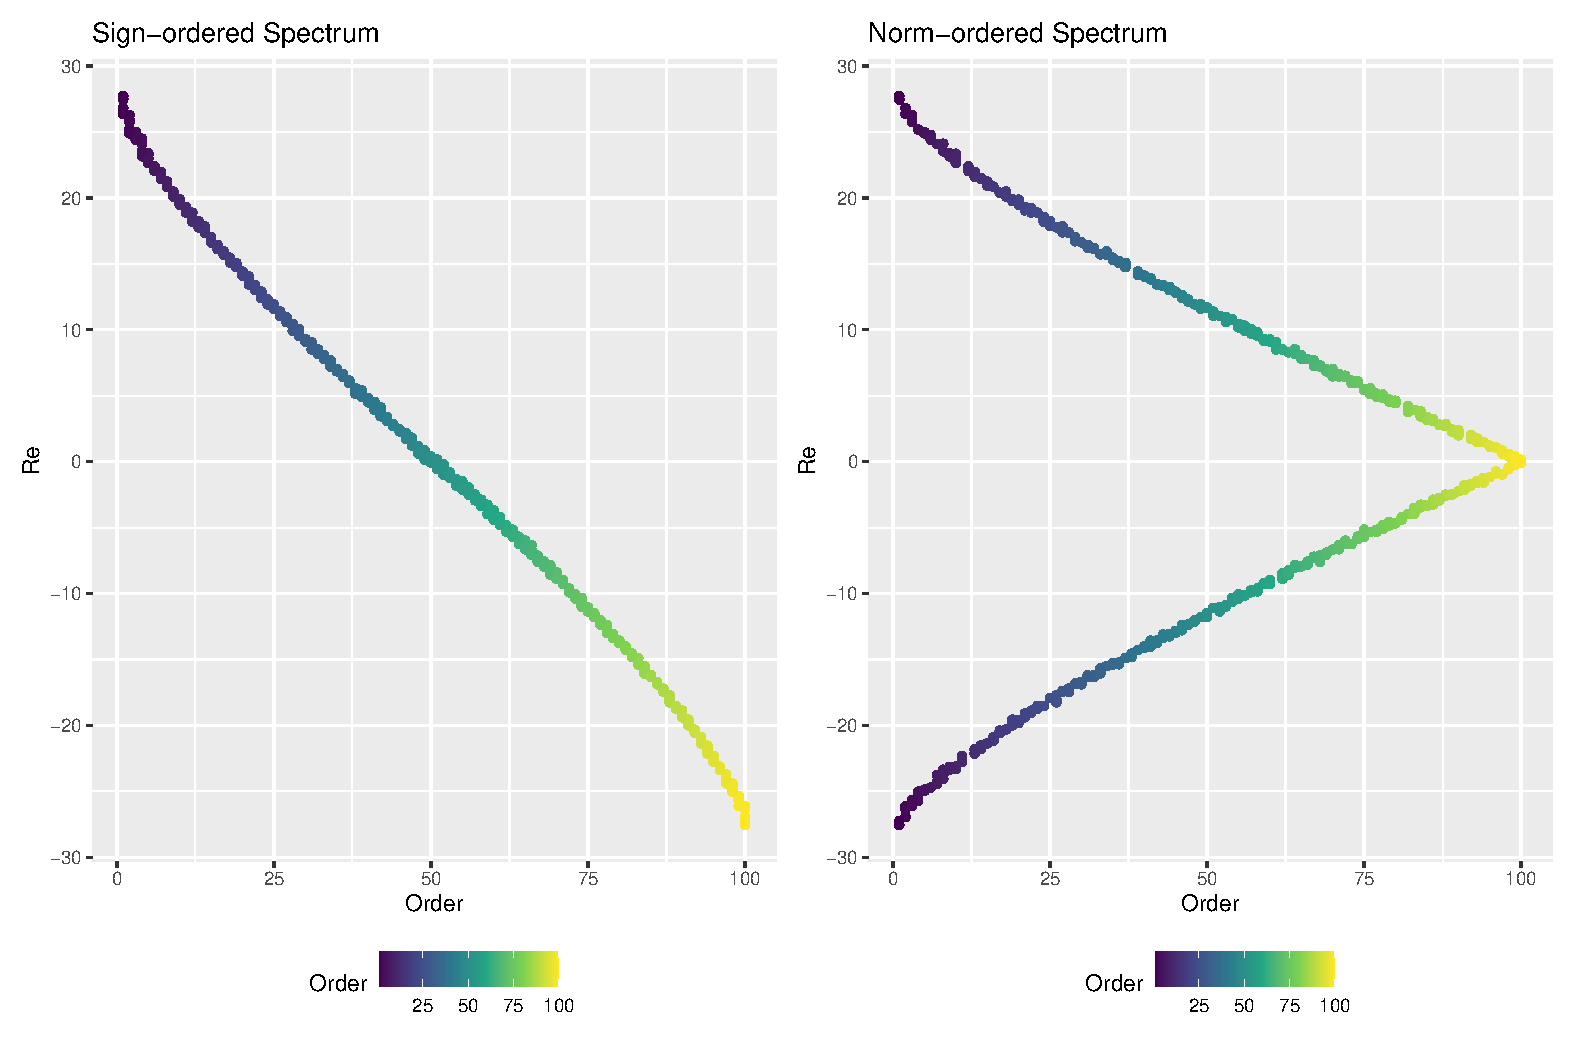
\includegraphics[scale = #2]{../graphics/chap2/2-2-1_orderscheme}
    \caption{Spectrum displaying two different ordering scheme}
   \end{center}
   \label{orderscheme_plot}
  \end{figure}
}

\newcommand{\FIGUREsemicircle}[2]{
  \begin{figure}[#1]
   \begin{center}
    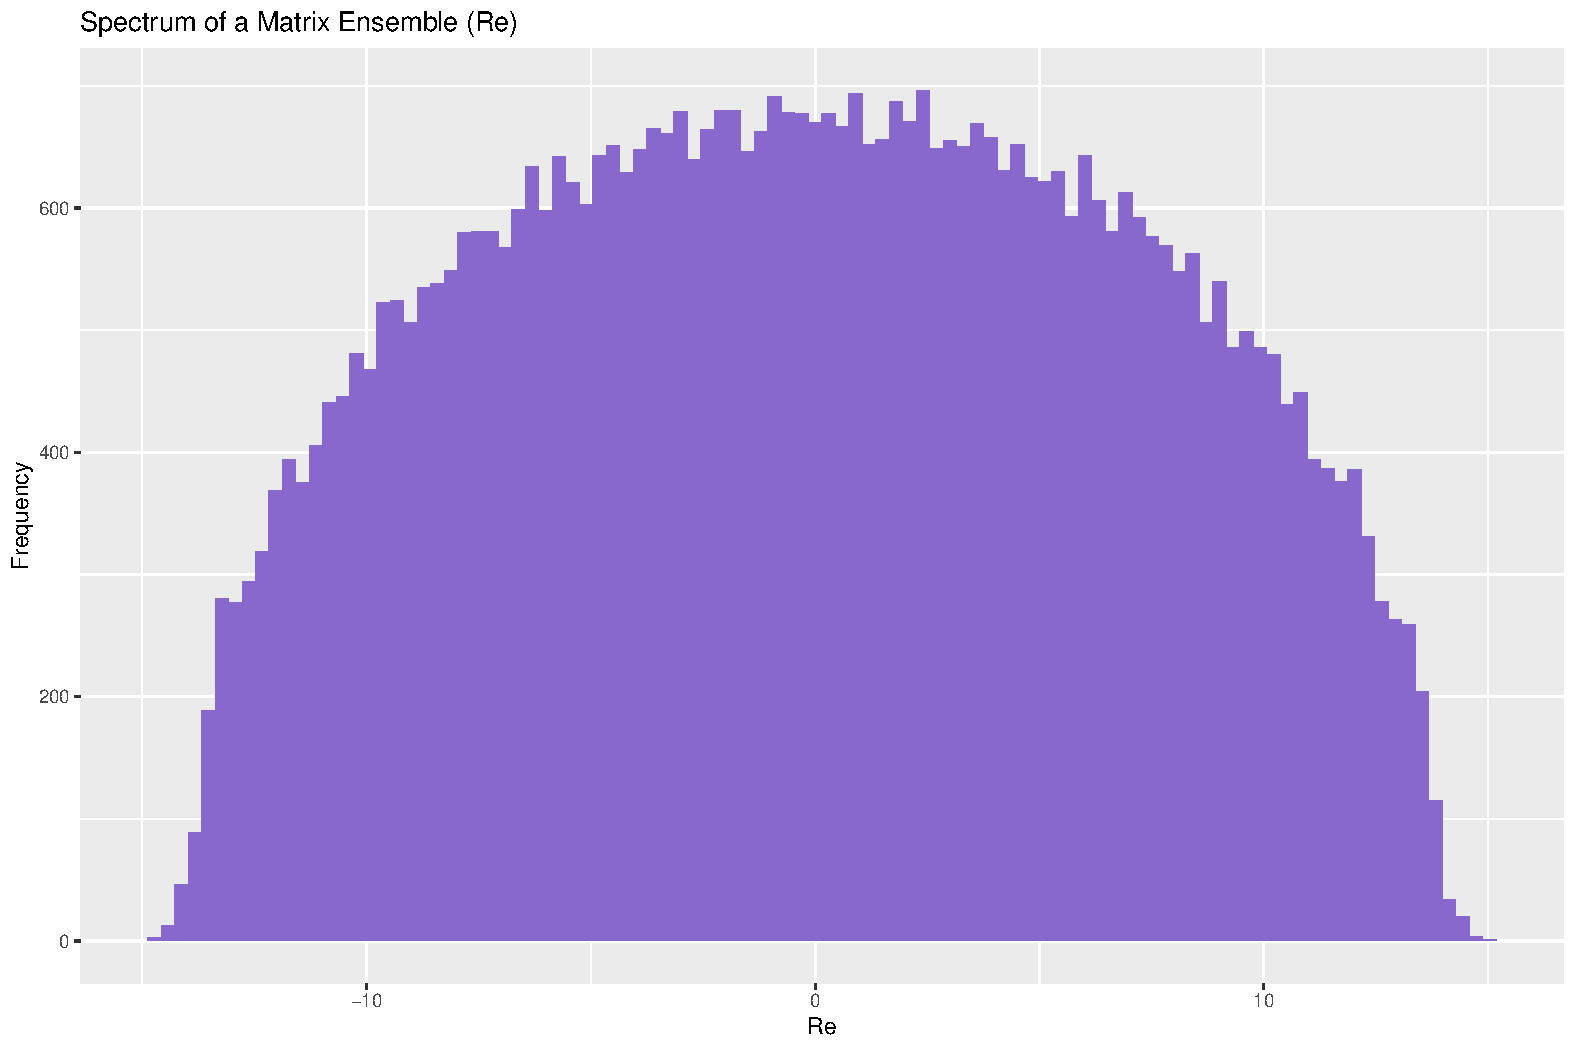
\includegraphics[scale = #2]{../graphics/chap2/2-3-2_semicircle}
    \caption{Eigenvalues of a Symmetric Matrix displaying the Semicircle Distribution}
   \end{center}
   \label{semicircleplot}
  \end{figure}
}
%==================
%     CHAPTER 3
%==================

%==================
%     CHAPTER 4
%==================s


%==================
%    ALGORITHS
%==================

%%%%%%%%%%%%%%%%%%%%%%%%%%%%%%%%%%%%%%%%%%%%%%%%%%%%%%%%%%%%%%%%%%%%%%%%%%%%%%%%%%%%%%%%%%%%%%%%
% 																	Implicit D-Matrices
%%%%%%%%%%%%%%%%%%%%%%%%%%%%%%%%%%%%%%%%%%%%%%%%%%%%%%%%%%%%%%%%%%%%%%%%%%%%%%%%%%%%%%%%%%%%%%%%

\newcommand{\ALGstochrow}{
	\begin{algorithm}[Stochastic Row] \hfill
	\begin{enumerate}
		\item To sample a row $r$ of size $N$, fix $N \in \N$.
		\item Sample a vector $\vec{X}$ with $N$ i.i.d entries between $[0,1]$. So, sample $\vec{X} \sim \Unif(0,1)$.
		\item Assign $r \la \vec{X}$, and then normalize the row by diving each entry by the row sum; so assign $r \la r \cdot \frac{1}{\sum_{i = 1}^N{r_i}}$
		\item Return the stochastic row $r$.
	\end{enumerate}
	\end{algorithm}
}

\newcommand{\ALGstoch}{
	\begin{algorithm}[Stochastic Matrix] \hfill
	\begin{enumerate}
		\item To generate a stochastic square matix $P$ of size $N$, fix $N \in \N$.
		\item Then, for every row of $P$, randomly sample a stochastic row and assign it to $P$.
		\item Return the stochastic matrix $P$.
	\end{enumerate}
	\end{algorithm}
}

\newcommand{\ALGstochsymm}{
	\begin{algorithm}[Symmetric Stochastic Matrix] \hfill
	\begin{enumerate}
		\item To sample a symmetric stochastic matrix $P$ of size $N$, fix $N \in \N$.
		\item Sample a random stochastic matrix $Q$ of size $N$.
		\item Choosing one of the triangles of $Q$, set both the upper and lower of triangles of $P$ to be that triangle.
		\item Set the diagonal of the matrix $P$ to be equal to 1 minus the sum of the non-diagonal entries.
		\item Return the symmetric stochastic matrix $P$.
	\end{enumerate}
	\end{algorithm}
}

\newcommand{\ALGerdos}{
	\begin{algorithm}[Transition Matrix for an Erdos-Renyi Graph] \hfill
	\begin{enumerate}
		\item{Fix $N \in \N$ and $p \in [0,1]$}.
		\item{Generate a matrix Q such that every entry $i,j\in \oneto[N]$ is $x_{ij} \sim \Unif(0,1)$.}
		\item{For each row $r_i$ in $\{1,\dots,N\}$, generate $deg(v_i) \sim \Bin(N,p)$.}
		\item{Randomly chose $N-deg(v_i)$ vertices, set the entries $x_{ij}$ in the $j$ columns to 0 to sever them.}
		\item{Renormalize the matrix by dividing each row by its sum; let $(x_i) \leftarrow (x_i)/\sum_j(x_i)$}.
	\end{enumerate}
	\end{algorithm}
}

%%%%%%%%%%%%%%%%%%%%%%%%%%%%%%%%%%%%%%%%%%%%%%%%%%%%%%%%%%%%%%%%%%%%%%%%%%%%%%%%%%%%%%%%%%%%%%%%
% 																	Explicit D-Matrices
%%%%%%%%%%%%%%%%%%%%%%%%%%%%%%%%%%%%%%%%%%%%%%%%%%%%%%%%%%%%%%%%%%%%%%%%%%%%%%%%%%%%%%%%%%%%%%%%

\newcommand{\ALGexplicit}{
	\begin{algorithm}[Homogenous Explicit $\D$-Matrix] \hfill
	\begin{enumerate}
		\item To simulate a $\D$-distributed square matrix $P$ of size $N$, fix $N \in \N$.
		\item Sample a vector $\vec{X}$ with $N$ i.i.d entries from $\D$. So, generate $\vec{X} = X_1,\dots,X_N \where X_i \text{is i.i.d } \D$.
		\item Assign the vector $\vec{X}$ as a row of the matrix $P$. Repeat for every other row.
		\item Return the $\D$-distributed matrix $P$.
	\end{enumerate}
	\end{algorithm}
}

\newcommand{\ALGbeta}{
  \begin{algorithm}[Dumitriu's Beta Matrix] \hfill
    \begin{enumerate}
      \item To simulate an $N \times N$ beta matrix, fix $N \in \N$.
      \item Start by taking a diagonal of $\Normal(0,2)$ variables.
      \item Set both of the nearest off-diagonals to the row that samples from a $\chi(df = c_j) \where c_j = \beta \cdot j$ for columns spanning $j = 1,\dots,n-1$.
    \end{enumerate}
  \end{algorithm}
}

\newcommand{\ALGbetaunnum}{
  \begin{algorithm*}[Dumitriu's Beta Matrix] \hfill
    \begin{enumerate}
      \item To simulate an $N \times N$ beta matrix, fix $N \in \N$.
      \item Start by taking a diagonal of $\Normal(0,2)$ variables.
      \item Set both of the nearest off-diagonals to the row that samples from a $\chi(df = c_j) \where c_j = \beta \cdot j$ for columns spanning $j = 1,\dots,n-1$.
    \end{enumerate}
  \end{algorithm*}
}

 % Input supporting TeX header files

%% Thesis Preamble
\title{Spectral Statistics of Random Matrices}
\author{Ali Taqi}
\date{May 2021}
\division{Mathematics and Natural Sciences}
\advisor{Jonathan M. Wells}
\department{Mathematics}

% TeX Settings
\setlength{\parskip}{0pt}
\setlength{\headheight}{15pt}

% The fun begins
\begin{document}
  \maketitle
  \frontmatter % this stuff will be roman-numbered
  \pagestyle{empty} % this removes page numbers from the frontmatter

%     \chapter*{Acknowledgements}
% 	For my mother.

%     \chapter*{Preface}
% 	This is an example of a thesis setup to use the reed thesis document class.

%     \chapter*{List of Abbreviations}
% 		You can always change the way your abbreviations are formatted. Play around with it yourself, use tables, or come to CUS if you'd like to change the way it looks. You can also completely remove this chapter if you have no need for a list of abbreviations. Here is an example of what this could look like:
%
% 	\begin{table}[h]
% 	\centering % You could remove this to move table to the left
% 	\begin{tabular}{ll}
% 		\textbf{ABC}  	&  American Broadcasting Company \\
% 		\textbf{CBS}  	&  Columbia Broadcasting System\\
% 		\end{tabular}
% 	\end{table}

    \tableofcontents

    \listoftables \hfill

    \begin{center}

    \Ddisttable \newline

    \hfill \vspace{2em}

    \spectrumschemetable \newline

    \hfill \vspace{2em}

    \dispersiontable \newline

    \hfill \vspace{2em}

    \pairingschemetable \newline

    \end{center}

%    \listoffigures

% If your abstract is longer than a page, there may be a formatting issue.
    \chapter*{Abstract}
	On their own, random variables exude deterministic properties regarding their uncertainty. The same generalization can be made for random matrices, which are matrices whose entries are random variables. One particular statistic worth investigating is the distribution of a matrix ensemble's eigenvalues, or its spectrum. In this thesis, there will be an exploration of various classes of random matrices and relevant spectral statistics like their spectra and mixing times.

	\chapter*{Dedication}
	For my mother.

  \mainmatter % here the regular arabic numbering starts
  \pagestyle{fancyplain} % turns page numbering back on

%The \introduction command is provided as a convenience.
%if you want special chapter formatting, you'll probably want to avoid using it altogether

  \chapter*{Introduction}
       \addcontentsline{toc}{chapter}{Introduction}
\chaptermark{Introduction}
\markboth{Introduction}{Introduction}
	
	% The three lines above are to make sure that the headers are right, that the intro gets included in the table of contents, and that it doesn't get numbered 1 so that chapter one is 1.
	
What are *spectral statistics*? Do they have to do with rainbows? Sceptres? No, they don't, but they're almost as colorful and regal. *Spectral statistics*, aptly named so, borrows from the spectral-like patterns observed in statistical physics - whether it may be atomic spectra or other quantum mechanical phenomena. The borrowing is loose and not literal, but still somewhat well founded. 

Random matrix theory - as a field - was developed extensively in the 1930s by Wigner, a nuclear physicist. He found connections between the deterministic properties of atomic nuclei and their random and stochastic behaviors. The link? -- Random matrices.   






% Double spacing: if you want to double space, or one and a half space, uncomment one of the following lines.
% You can go back to single spacing with the \singlespacing command.
% \onehalfspacing
% \doublespacing

% Beginning of Chapters

\chapter{Random Matrices}

%=========================================================================================
\epigraph{Unfortunately, no one can be told what The Matrix is. You'll have to see it for yourself.}{\textit{Morpheus \\ The Matrix}}
%=========================================================================================

As discussed in the introduction, this thesis will be an exploration of spectral statistics of random matrices. This means that we must first be able to understand what random matrices are. At a fundamental level, random matrices are simply matrices whose entries are randomly distributed in accordance to some distribution or method. To formalize all these notions, we will define what random matrices are and what it means for them to be $\D$-distributed.

Prior to beginning the discussion on $\D$-distributions, the reader should be familiar or at least accquainted with the notion of random variables and what they are. A summary is available in the appendix in A.x.

%\section{Introduction}
When it comes to random simulation, there must always be a rule to which our randomness must conform, regardless of complexity. For example, sampling a vector from a distribution is a rudimentary example of this. For random matrices, there will be a few methods of generating their entries that are not just sampling from theoretical distributions. As such, we motivate the $\D$-distribution.

%=========================================================================================
%=========================================================================================

\section{$\D$-Distributions}

Now, we motivate the $D$-distribution. A formalization on how to initialize a random matrix.

\begin{definition}[$\D$-distribution]
When we define a random matrix that is $\D$-distributed, we say that $P \sim \D$. In the simplest of terms, $\D$ is essentially the algorithm that generates the random matrix $P$. We define two primary methods of distribution: explicit distribution and implicit distribution. If $\D$ is an explicit distribution, then every entry of $P$ is homogenously sampled from that distribution. Otherwise, if it is implicit, we utilize an algorithm that imposes an implicit distribution on the entries.
\end{definition}

%=========================================================================================

\subsection{Explicit Distributions}

The simplest case is homogenous, explicitly distributed random matrices. If $\D$ is an explicit distribution, then we overload the notation $\D$ to mean a probability distribution in the classical sense (see Appendix A.x). So, if $\D$ is a probability distribution, the matrix $P \sim \D$ when $p_{ij} \sim \D$. In otherwords, we simply perform entry-wise sampling from that distribution.

Take for example the following explicit distributions which we cover in this thesis.

\begin{enumerate}
\item  If $\D = \Normal(0,1)$, then $p_{ij} \sim \Normal(0,1)$.
\item  If $\D = \Unif(0,1)$, then $p_{ij} \sim \Unif(0,1)$.
\end{enumerate}

\begin{formalization}
Explicit distributions can be formalized in scope of the standard notation in probability theory. At the heart of the formalization is the usage of index hacking to collapse the array's indices from two dimensions to one. This way, our random matrix has a representation as a random vector, which we commonly encounter in probability theory as a (i.i.d) sequence of random variables! Generally, an $N \times N$ random matrix that is explicity and homogenously $\D$-distributed is essentially a sequence of $N^2$ i.i.d random variables sampled from $\D$.
\end{formalization}

\begin{example}[Formalization]
For example, suppose $P$ is a $2 \times 2$ random matrix with $\D = \Normal(0,1)$. Then, we have four random variables to initialize. In the random matrix representation, we need to initialize $P_{11}, P_{12}, P_{21}, \and P_{22}$ by sampling them from $\D$. In the vector representation, we just say we are sampling four i.i.d random variables from $\D$. The matrix indexing is intrinsic and preservable by using index hacking with some modular math.
\end{example}

%=========================================================================================

\subsection{Implicit Distributions}

In the latter case, we are concerned less about the distribution of the matrix entries and moreso about its holisitic properties.

Consider for example, the following implicit distributions.

\begin{enumerate}
\item If $\D = \text{Stochastic}$, then the matrix is a row of random stochastic rows. (See Algorithm B.x)
\item If $\D$ is any distribution (implicit or explicit), then $\D^{\dagger}$ is the Symmetric/Hermitian version of $\D$. (See Algorithm B.x)
\end{enumerate}

%=========================================================================================

\subsection{Random Matrices}

With $\D$-distributions defined, we may finally define a random matrix.

\begin{definition}[Random Matrix]
Assuming $\D$ is an explicit distribution, a random matrix is any matrix over the field $\F$ is a matrix $M \in \F^{N \times N}$ is a matrix whose entries are i.i.d random variables. So, if a random matrix $M = (m_{ij})$ is $\mathcal{D}$-distributed, then we say $m_{ij} \sim \mathcal{D}$. In the scope of this thesis, assume every random matrix to be homogenously distributed. Otherwise, if $\D$ is an implicit distribution, then $P$ is a matrix whose entries are determined by the algorithm imposed by $\D$.
\end{definition}

\noindent Sometimes, we want our matrix to have complex entries. We notate this by specifying $\F = \Cc$.

\begin{remark}[Complex Entries]
To say that a random matrix is explicitly $\D$-distributed over $\Cc$ would mean that its entries take the form $a + bi$ where $a,b \sim \D$ are random variables. In other words, if we allow the matrix to have complex entries by setting $\F = \Cc$, then we must sample the real and imaginary component as $\D$-distributed i.i.d. random variables.
\end{remark}

\medskip
\noindent Below, we can see code on how to generate a standard normal random matrix using the $\textbf{RMAT}$ package.
\begin{code}[Standard Normal Matrix]
Let $\mathcal{D} = \Normal(0,1)$. We can generate $P \sim \D$, a $4 \times 4$ standard normal matrix, as such:
\end{code}

\begin{lstlisting}[language=R]
library(RMAT)
P <- RM_norm(N = 4, mean = 0, sd = 1)
# Outputs the following
P
           [,1]       [,2]       [,3]        [,4]
[1,]  0.1058257 -1.0835598 -0.7031727  1.01608625
[2,] -0.2170453  1.8206070 -0.4539230  0.06828296
[3,]  1.3002145  0.1254992 -0.5214005 -0.61516174
[4,] -1.0398587  0.1975445 -0.8511950  0.86366082
\end{lstlisting}

%****************************************************************************************%
\minititle{Summary Table of $\D$-Distributions}
\begin{center}
  \Ddisttable
\end{center}
%****************************************************************************************%
\newpage

%=========================================================================================
%=========================================================================================

\section{The Crew: Ensembles}

With a random matrix well defined, we may now motivate one of the most important ideas - the random matrix ensemble. One common theme in this thesis will be that random matrices on their own provide little information. When we consider them at the ensemble level, we start to obtain more fruitful results. Without further ado, we motivate the random matrix ensemble.

\begin{definition}[Random Matrix Ensemble]
A $\D$-distributed random matrix ensemble $\Ens$ over $\F^{N \times N}$ of size $K$ is defined as a set of $\D$-distributed random matrices $\Ens = \{P_i \sim \mathcal{D} \mid P_i \in \F^{N \times N}\}_{i = 1}^K$. In simple words, it is simply a collection of $K$ iterations of a specified class of random matrix.
\end{definition}

\medskip
\noindent So, for example, we could compute a simple ensemble of matrices as follows.
\begin{code}[Standard Normal Hermitian Ensemble]
Let $\mathcal{D} = \Normal(0,1)^{\dagger}$. We can generate $\Ens \sim \D$ over $\Cc$, an ensemble of $4 \times 4$ complex Hermitian standard normal matrices of size 10 as such:
\end{code}

\begin{lstlisting}[language=R]
library(RMAT)
# By default, mean = 0 and sd = 1.
ensemble <- RME_norm(N = 4, cplx = TRUE, herm = TRUE, size = 10)
# Outputs the following
ensemble
...
[[10]]
                  [,1]              [,2]              [,3]
[1,] -0.59931+1.24286i  1.29457+0.66058i  0.83539-0.16662i
[2,]  1.29457-0.66058i  0.78841+0.09818i -1.16592+1.14666i
[3,]  0.83539+0.16662i -1.16592-1.14666i -0.51256+0.17750i
\end{lstlisting}

With this in mind, we will gloss over, characterize, and briefly discuss a few special recurring ensembles in this thesis.

%=========================================================================================

\subsection{Erdos-Renyi $p$-Ensembles}

The Hermite $\beta$-ensembles are a normal-like class of random matrices. Now, we will veer away from the normal distribution as a whole and switch to a different class of matrices: stochastic matrices. Stochastic matrices, in short, are matrices that represent Markov Chains (see A.x). We can also think of them as the matrix representation of a specific setup of a walk on a random graph.

A particular class of random graphs that we will consider are the Erdos-Renyi random graphs. Essentially, these are graphs whose vertices are connected with a uniform probability $p$. We can interpret this as saying an Erdos-Renyi graph is a simple random walk on a graph with parameterized sparsity (given by $p$). Without further ado, we motivate the Erdos-Renyi graph:

\begin{definition}[Erdos-Renyi Graph]
An Erdos-Renyi graph is a graph $G = (V,E)$ with a set of vertices $V = \{\oneto[N]\}$ and edges $E = \mathds{1}_{i,j \in V} \sim \Bern(p_{ij})$. It is homogenous if $p_{ij} = p$ is fixed for all $i, j$.
\end{definition}

Essentially, an Erdos-Renyi graph is a graph whose 'connectedness' is parameterized by a probability $p$ (assuming it's homogenous, which this document will unless otherwise noted). As $p \to 0$, we say that graph becomes more sparse; analogously, as $p \to 1$ the graph becomes more connected.\newline
\indent Recall from probability theory that a sum of i.i.d Bernoulli random variables is a Binomial variable. As such, we may alternatively say that the degree of each vertex $v$ is distributed as $deg(v) \sim Bin(N,p)$ where $N$ is the number of vertices. This makes simulating the graphs much easier.

\begin{code}[Erdos-Renyi p = 0.5 Ensemble]
Let $\mathcal{D} = \text{ER}(p = 0.5)$. We can generate $\Ens \sim \D$, an ensemble of $4 \times 4$ Erdos-Renyi matrices ($p = 0.5$) of size 10 as such:
\end{code}

\begin{lstlisting}[language=R]
library(RMAT)
ensemble <- RME_erdos(N = 4, p = 0.5, size = 10)
# Outputs the following
ensemble
...
[[10]]
          [,1]      [,2]      [,3]     [,4]
[1,] 0.0000000 0.1729581 0.8270419 0.000000
[2,] 0.0000000 0.0000000 1.0000000 0.000000
[3,] 0.2557890 0.3766740 0.0000000 0.367537
[4,] 0.2151029 0.3929580 0.3919391 0.000000
\end{lstlisting}

%=========================================================================================

\subsection{Hermite $\beta$-Ensembles}

The Hermite $\beta$-Ensembles will be one of the primary ensembles discussed in this thesis. This ensemble will be characterized, motivated, and defined more thoroughly in $\textbf{Chapter 4}$. However, we will give a brief introduction to the ensemble.

At a practical level, all one would need to know is that the matrices are generated in accordance to an algorithm found in the appendix (Algorithm B.x) and in Chapter 4.

%=========================================================================================

%\section{Analytical Results}


\chapter{Spectra}

%%%%%%%%%%%%%%%%%%%%%%%%%%%%%%%%%%%%%%%%%%%%%%%%%%%%%%%%%%%%%%%%%%%%%%%%%%%%%%%%%%%%%%%%%%
\epigraph{Life is like a box of crayons.}{\textit{Unknown}}
%%%%%%%%%%%%%%%%%%%%%%%%%%%%%%%%%%%%%%%%%%%%%%%%%%%%%%%%%%%%%%%%%%%%%%%%%%%%%%%%%%%%%%%%%%

\section{Introduction}
So, what are \textit{spectral statistics}? Do they have to do with rainbows? Sceptres? No, they don’t, but they’re almost as colorful and regal. The word spectral is borrowed from the spectral-like patterns observed in statistical physics - whether it may be atomic spectra or other quantum mechanical phenomena. The borrowing is loose and not literal, but still somewhat well founded. In fact, the field of Random Matrix Theory was extensively developed in the 1930s by the nuclear physicist Eugene Wigner. He found connections between the deterministic properties of atomic nuclei and their random and stochastic behaviors. The link? Random matrices. \newline

So in the context of this thesis, \textit{spectral statistics} will be an umbrella term for random matrix statistics that somehow involve that matrix's eigenvalues and eigenvectors. That being said, if we fix a \textit{random matrix}, we can study its features by studying its eigenvalues - fundemental numbers that tell us a lot about the matrix. They are quite important for many reasons. For instance in statistical physics, many processes are represented by operators or matrices, and as such, their behaviours could be partially determined by the eigenvalues of their corrosponding matrices. The study of eigenvalues and eigenvectors primarily falls in the scope of Linear Algebra, but their utility is far-reaching. So, what exactly are \textit{eigenvalues} exactly?

%%%%%%%%%%%%%%%%%%%%%%%%%%%%%%%%%%%%%%%%%%%%%%%%%%%%%%%%%%%%%%%%%%%%%%%%%%%%%%%%%%%%%%%%%%

\subsection{The Quintessential Spectral Statistic: the Eigenvalue}
Given any standard square matrix $P \in \F^{N \times N}$, its \textit{eigenvalues} are simply the roots of the characteristic polynomial $\text{char}_P{(\lambda)}$ = $\det(P - \lambda I)$. By the Fundamental Theorem of Algebra, we know that there is always have as many complex eigenvalues $\lambda \in \Cc$ as the dimension of the matrix.

That being said, when our random matrix has a specified distribution (say, standard normal), we can see patterns in the eigenvalue distributions. So, an eigenvalue is a \textbf{spectral statistic} of a random matrix! To talk about a matrix's eigenvalues in a more formal and concise manner, we motivate what is the \text{eigenvalue spectrum}.

\newpage

\begin{definition}[Spectrum]
Suppose $P \in \F^{N \times N}$ is a square matrix of size $N$ over $\F$. Then, the (eigenvalue) spectrum of $P$ is defined as the multiset of its eigenvalues and it is denoted
$$\sigma(P) = \{\lambda_i \in \Cc \mid \text{char}_P(\lambda_i) = 0 \}_{i=1}^N$$
Note that it is important to specify that a spectrum is a multiset and not just a set; eigenvalues could be repeated due to algebraic multiplicity and we opt to always have $N$ eigenvalues.
\end{definition}

\medskip
\noindent For example, consider the following code example from the RMAT package.
\begin{code}[Spectrum of a Standard Normal Matrix]
Let $P \sim \Normal(0,1)$ be a $4 \times 4$ standard normal random matrix. We can generate the spectrum of $P$, $\sigma(P)$ as follows:
\end{code}

\begin{lstlisting}[language=R]
library(RMAT)
P <- RM_norm(N = 5, mean = 0, sd = 1)
spectrum_P <- spectrum(P)
# Outputs the following
spectrum_P
...
        Re      Im   Norm Order
 1 -0.5434  1.3539 1.4589     1
 2 -0.5434 -1.3539 1.4589     2
 3  0.2255  1.4250 1.4427     3
 4  0.2255 -1.4250 1.4427     4
 5 -0.8678  0.0000 0.8678     5
\end{lstlisting}

While our definition for spectrum is nice and clean, there are a few caveats that we must take care of. First, how are spectra statistics? So we can even call them statistics, so there needs to be some formalization as to why we consider eigenvalues statistics. In this dialogue, we will call back on the same sort of formalization dialogue in the Random Matrices section. Before beginning, the reader is encouraged to review what a statistic is in the review appendix (A.x).

Recall that when we defined and motivated the $\D$-distribution framework of simulating random matrices,we always had one thing - a vector representation of random variables. Using this framework, the formalization is trivial.

\begin{formalization}
Suppose $P \sim \D$ is an $N \times N$ random matrix. Then, $P$ has a representation as a sequence of $N^2$ random variables, denote it $\vec{X} = \{X_i \mid i = 1,2,\dots,N^2 - 1,N^2\}$. Then, the spectrum of the matrix $P$ is simply a function of the vector $\vec{X}$. We can denote this $\sigma(\vec{X})$, where the operator $\sigma$ is overloaded to mean the spectrum of a matrix $\textbf{with respect to the vector representation}$. The actual process for $\sigma$ is not necessary to explicitly write out, since characterizing it will be sufficient for now. Essentially, $\sigma$ is a function that would parse the random variables into the array form by index hacking. Then, it must compute the determinant of the matrix $P - \lambda I$, and solve for its roots. To summarize this, consider the flow chart below.
\end{formalization}

To summarize, here is how we formalize the spectrum as a statistic. Suppose we sample $P \sim \D$. Then, we take its spectrum formally using $\sigma$ as such:\hfill
$$P_{\text{array}} \ra \vec{P} \ra \sigma(\vec{P}) \ra \text{index magic} \ra \det(P - \lambda I) \ra \sigma(P_{\text{array}})$$

%%%%%%%%%%%%%%%%%%%%%%%%%%%%%%%%%%%%%%%%%%%%%%%%%%%%%%%%%%%%%%%%%%%%%%%%%%%%%%%%%%%%%%%%%%

\subsection{Interlude: Ensembles}
While the spectrum of a matrix provides a good summary of the matrix, a matrix is only considered a single point/observation in random matrix theory. Additionally, simulating large matrices and computing their eigenvalues becomes harder and more computationally expensive as $N \to \infty$. As such, to obtain more eigenvalue statistics efficiently, another dimension is introduced by motiving the \textit{spectrum of a random matrix ensemble}. If we have an ensemble $\Ens$, then we can naturally extend the definition of $\sigma(\Ens)$.

\begin{definition}[Ensemble Spectrum]
Let $\Ens \sim \D$ be an ensemble of matrices $P_i \in \F^{n \times n}$. To take the spectrum of $\Ens$, simply take the union of the spectra of each of its matrices. In other words, if $\Ens = \{P_i \sim \mathcal{D}\}_{i = 1}^K$, then we denote the spectrum of the ensemble
$$\sigma(\Ens) = \bigcup_{i=1}^K \sigma(P_i)$$
\end{definition}

\medskip
\noindent For example, consider the following code example from the RMAT package.
\begin{code}[Spectrum of a Standard Normal Matrix Ensemble]
Let $\Ens \sim \Normal(0,1)$ be an ensemble of $3 \times 3$ standard normal random matrices of size $3$. We can generate the spectrum of $\Ens$, $\sigma(\Ens)$ as follows:
\end{code}

\begin{lstlisting}[language=R]
library(RMAT)
ens <- RME_norm(N = 3, mean = 0, sd = 1, size = 3)
spectrum_ens <- spectrum(ens)
# Outputs the following
spectrum_ens
...
        Re      Im   Norm Order
 1  1.7581  0.0000 1.7581     1
 2 -0.2614  1.0012 1.0347     2
 3 -0.2614 -1.0012 1.0347     3
 4  1.2327  0.4227 1.3032     1
 5  1.2327 -0.4227 1.3032     2
 6 -0.8504  0.0000 0.8504     3
 7 -0.5296  1.0508 1.1767     1
 8 -0.5296 -1.0508 1.1767     2
 9  0.7357  0.0000 0.7357     3
\end{lstlisting}

A common theme in this thesis will be that singleton matrices do not provide insightful information on their own. Rather, it is the collective behavior of a $\D$-distributed ensemble that tells us about how $\D$ impacts our spectral statistics. So in a way, ensemble statistics are the engine of this research.

%FFFFFFFFFFFFFFFFFFFFFFFFFFFFFFFFFFFFFFFFFFFFFFFFFFFFFFFFFFFFFFFFFFFFFFFFFFF
\FIGUREspectrumcomparison{h}{0.65}
%FFFFFFFFFFFFFFFFFFFFFFFFFFFFFFFFFFFFFFFFFFFFFFFFFFFFFFFFFFFFFFFFFFFFFFFFFFF

%%%%%%%%%%%%%%%%%%%%%%%%%%%%%%%%%%%%%%%%%%%%%%%%%%%%%%%%%%%%%%%%%%%%%%%%%%%%%%%%%%%%%%%%%%
%%%%%%%%%%%%%%%%%%%%%%%%%%%%%%%%%%%%%%%%%%%%%%%%%%%%%%%%%%%%%%%%%%%%%%%%%%%%%%%%%%%%%%%%%%
\newpage
\section{Spectrum Analysis}

%%%%%%%%%%%%%%%%%%%%%%%%%%%%%%%%%%%%%%%%%%%%%%%%%%%%%%%%%%%%%%%%%%%%%%%%%%%%%%%%%%%%%%%%%%

\subsection{Ordered Spectra}

\minititle{Order Schemes: How to Order Eigenvalues}

When we motivate the idea of matrix dispersion in the next section, we will consider order statistics of that matrix's eigenvalues in tandem with its dispersion. However, to do so presupposes that we have a sense of what \textit{ordered} eigenvalues means. Take a matrix $P$ and its \textit{unordered} spectrum $\sigma(P) = \{\lambda_j\}$. It is paramount to know what ordering scheme $\sigma(P)$ is using, because otherwise, the eigenvalue indices are meaningless! So, to eliminate confusion, we add an index to $\sigma$ that indicates how the spectrum is ordered. Often, the ordering context will be clear and the indexing will be omitted. Consider the two following $\textit{ordering schema}$:

Standard definitions of an ordered spectrum follows the standard ordering in the reals; denote this as the ordering by the $\textbf{sign scheme}$. Note that because total-ordering is only well-defined on the reals, we can only use this scheme when on a spectrum with real entries. So, we write the $\textit{sign-ordered spectrum}$ as follows:
\begin{align*}
\sigma_S(P) = \{\lambda_j : \lambda_1 \geq \lambda_2 \geq \dots \geq \lambda_N\}_{j = 1}^N
\end{align*}
Alternatively, we can motivate a different scheme that properly handles complex eigenvalues. We could sort the spectrum by the norm of its entries; denote this as ordering using the \textit{norm scheme}. This way, all the eigenvalues are mapped to a real value, in which we could use the sign-scheme of ordering. Without further ado, we write the $\textit{norm-ordered spectrum}$ as follows:
\begin{align*}
\sigma_N(P) = \{\lambda_j : |\lambda_1| \geq |\lambda_2| \geq \dots \geq |\lambda_N|\}_{j = 1}^N
\end{align*}
Note that when we take the norms of the eigenvalues, we essentially ignore "rotational" features of the eigenvalues. Signs of eigenvalues indicate reflection or rotation, so when we take the norm, we essentially become more concerned with scaling.

For example, consider the following plots, showing the difference in using the sign and norm ordering schemes for the same spectrum.

%FFFFFFFFFFFFFFFFFFFFFFFFFFFFFFFFFFFFFFFFFFFFFFFFFFFFFFFFFFFFFFFFFFFFFFFFFFF
\FIGUREorderscheme{h}{0.55}
%FFFFFFFFFFFFFFFFFFFFFFFFFFFFFFFFFFFFFFFFFFFFFFFFFFFFFFFFFFFFFFFFFFFFFFFFFFF

%%%%%%%%%%%%%%%%%%%%%%%%%%%%%%%%%%%%%%%%%%%%%%%%%%%%%%%%%%%%%%%%%%%%%%%%%%%%%%%%%%%%%%%%%%
\newpage
\minititle{Singular Values}

An aternative to using the norm ordering scheme is using the singular values of the matrix. If a matrix is symmetric, the singular values are simply the norm of the eigenvalues. We ignore rotational features and focus solely on scale when we do so.

Suppose $P$ is a random matrix. Then, we can take it singular values as such.

\begin{definition}[Singular Values]
The singular values of a matrix $P$ are given by the square root of the eigenvalues of the corrosponding product of that matrix and its transpose. That is, $\sigma_+(P) = \sqrt{\sigma(P \cdot P^T)}$.
\end{definition}


%\newpage
%****************************************************************************************%
\minititle{Summary Table of Spectrum Schema}
\spectrumschemetable
%****************************************************************************************%

%%%%%%%%%%%%%%%%%%%%%%%%%%%%%%%%%%%%%%%%%%%%%%%%%%%%%%%%%%%%%%%%%%%%%%%%%%%%%%%%%%%%%%%%%%

\minititle{Order Statistics}

With eigenvalue ordering unambiguous and well-defined, we may proceed to start talking about their order statistics. In short, given a random sample of fixed size, order statistics are random variables defined as the value of an element conditioning on its rank within the sample. (See A.x)

In general, order statistics are quite useful and tell us a lot about how the eigenvalues distribute given a distribution. They tell us how the eigenvalues space themselves and give us useful upper and lower bounds.

For example, the maximum of a sample is an order statistic concerned with the highest ranked element. In our case, this could corrospond the largest eigenvalue of a spectrum. After all, a spectrum is a random sample of fixed size, so this statistic is well-defined.

\begin{example}[The Largest Eigenvalue]
Suppose we have seek the largest eigenvalue distribution for a ensemble distribution $\D$, we would simulate an ensemble $\Ens$ and observe $\lambda_1$ for each of its matrices. Then, we can set the distribution of the largest eigenvalue for $\D$ by observing the distribution of $\lambda_1$.
\end{example}

So, we fill consider the conditional order statistics $\E(\lambda_{i} \mid i)$ and $\Var(\lambda_{i} \mid i)$.

%%%%%%%%%%%%%%%%%%%%%%%%%%%%%%%%%%%%%%%%%%%%%%%%%%%%%%%%%%%%%%%%%%%%%%%%%%%%%%%%%%%%%%%%%%
%%%%%%%%%%%%%%%%%%%%%%%%%%%%%%%%%%%%%%%%%%%%%%%%%%%%%%%%%%%%%%%%%%%%%%%%%%%%%%%%%%%%%%%%%%
%\section{Spectrum Analysis}
\newpage
\subsection{Case Study: Perron-Frobenius Theorem}

\begin{definition}[Spectral Radius]
  Let be $P$ be any matrix and $\spec(P)$ be its ordered spectrum. Then, the spectral radius of $P$ is defined as $\rho(P) = ||\sup \spec(P)||$ is the norm of its largest eigenvalue.
\end{definition}

\minititle{Detour: The Perron-Frobenius Theorem}

Using the toolkit we have now accquired, we can now discuss an elegant, visual representation of the Perron-Frobenius theorem (See A.x). To put it shortly, the Perron-Frobenius theorem, applied to stochastic matrices is a result that gurantees a stationary distribution to an ergodic Markov Chain (see A.x). Sparing the details, we can use the conjunction of two facts, that if true, yield the result for the Perron-Frobenius Theorem for ergodic Markov chains through stochastic matrices.
\begin{enumerate}
  \item The largest eigenvalue of stochastic matrices is 1.
  \item When multiplied by $P^K$ (for large $K$), any point $v$ enters the eigenspace of the matrix's largest eigenvalue. That is, $v P^K$ is an eigenvector of $P$.
\end{enumerate}

Again, those two statements were not formally proven in this thesis. However, there are large amounts of computational evidence for both of these results. Consider the first statement.

Below we have a stochastic ensemble spectrum. Notice how the largest eigenvalue is 1, living far from the island of \textbf{complex} eigenvalues.

%FFFFFFFFFFFFFFFFFFFFFFFFFFFFFFFFFFFFFFFFFFFFFFFFFFFFFFFFFFFFFFFFFFFFFFFFFFF
\FIGUREstochspectrum{h}{0.65}
%FFFFFFFFFFFFFFFFFFFFFFFFFFFFFFFFFFFFFFFFFFFFFFFFFFFFFFFFFFFFFFFFFFFFFFFFFFF

This shows that the spectral of stochastic matrices is $1$! What is left is the other fact. For the second statement, again, there is plenty of computational evidence to back this up. This is the reason why \textbf{Appendix D} is included. This is a side project that started in this thesis, simulating eigenvectors computationally. From the simulations, we find that there is overwhelming evidence that most matrices, if not all, satisfy the second statement.

\blocktitle{Conclusions} So, to conclude, we can say that the computational evidence for these two facts support and provide an alternative method of seeing why the Perron-Frobenius theorem is true.

%%%%%%%%%%%%%%%%%%%%%%%%%%%%%%%%%%%%%%%%%%%%%%%%%%%%%%%%%%%%%%%%%%%%%%%%%%%%%%%%%%%%%%%%%%
%%%%%%%%%%%%%%%%%%%%%%%%%%%%%%%%%%%%%%%%%%%%%%%%%%%%%%%%%%%%%%%%%%%%%%%%%%%%%%%%%%%%%%%%%%
\newpage
\section{Symmetric and Hermitian Matrices}

%\subsection{Introduction}
A very important class of matrices in Linear Algebra is that of Symmetric or Hermitian matrices (See A.x). Simply put, those are matrices which are equal to their conjugate transpose.

$\textbf{Note:}$ Since real numbers are their own conjugate transpose, every Symmetric matrix is Hermitian. However, we will still delineate the two terms to avoid confusion.

In any case, one critical result in Linear Algebra that will be extensively wielded in this thesis is the fact that a matrix is Symmetric or Hermitian if and only if it has real eigenvalues. In other words:
\begin{align*}
P = \overline{P^{T}} \implies \sigma(P) = \{\lambda_i \mid \lambda_i \in \R\}
\end{align*}
Having a complete set of real eigenvalues yields many great properties. For instance, if all eigenvalues are real, we have the option of observing either the sign-ordered spectrum or the norm-ordered spectrum. This way, we can preserve negative signs and we would not lose the rotational aspect of the eigenvalue when we study its statistics. That is just one reason out of many more why having real eigenvalues is quite nice.

%%%%%%%%%%%%%%%%%%%%%%%%%%%%%%%%%%%%%%%%%%%%%%%%%%%%%%%%%%%%%%%%%%%%%%%%%%%%%%%%%%%%%%%%%%
\minititle{Example: Stochastic Matrices}

One very pleasing example to look at is stochastic matrices. As seen previously in \textbf{Section 2}, stochastic matrices tend to have two components: a complex disk of eigenvalues about the origin and singularity that is the largest eigenvalue.

Below we have a \textbf{symmetric} stochastic ensemble spectrum. Notice how the largest eigenvalue is 1, living far from the island of \textbf{real} eigenvalues. This can be compared to the spectrum of non-Symmetric stochastic matrices in the previous figure. The patterns are similar, but now, imposing symmetry on the matrices forces the eigenvalues to ``collapse'' onto the real line!

%FFFFFFFFFFFFFFFFFFFFFFFFFFFFFFFFFFFFFFFFFFFFFFFFFFFFFFFFFFFFFFFFFFFFFFFFFFF
\FIGUREsymmstochspectrum{h}{0.65}
%FFFFFFFFFFFFFFFFFFFFFFFFFFFFFFFFFFFFFFFFFFFFFFFFFFFFFFFFFFFFFFFFFFFFFFFFFFF

%%%%%%%%%%%%%%%%%%%%%%%%%%%%%%%%%%%%%%%%%%%%%%%%%%%%%%%%%%%%%%%%%%%%%%%%%%%%%%%%%%%%%%%%%%
\newpage
\subsection{Wigner's Semicircle Distribution}

The eigenvalues of Hermitian matrices obey Wigner's Semicircle distribution. Since Hermitian matrices have real eigenvalues, then we can be more precise and generally say that the real component of the eigenvalues follow the semicircle distribution. The distribution is named after physicist Eugene Wigner.

\begin{definition}[Semicircle Distribtion]
If a random variable $X$ is semicircle distributed with radius $R \in \R^+$, then we say $X \sim \text{SC}(R)$. $X$ has the following probability density function:
$$\Prb(X = x) = \frac{2}{\pi R^2} \sqrt{R^2 - x^2} \for x \in [-R, R]$$
\end{definition}

\begin{remark}[Radius and Matrix Dimension]
The dimension of the matrix determines the radius of the eigenvalues. Namely, if a Hermitian matrix $P$ is $N \times N$, then its eigenvalues are semicircle distributed with radius $R = 2\sqrt{N}$. That is, $P^{\dagger}$ has a spectrum $\sigma({P}) \sim \text{SC}(2\sqrt{R})$.
\end{remark}

%FFFFFFFFFFFFFFFFFFFFFFFFFFFFFFFFFFFFFFFFFFFFFFFFFFFFFFFFFFFFFFFFFFFFFFFFFFF
\FIGUREsemicircle{h}{0.6}
%FFFFFFFFFFFFFFFFFFFFFFFFFFFFFFFFFFFFFFFFFFFFFFFFFFFFFFFFFFFFFFFFFFFFFFFFFFF

%%%%%%%%%%%%%%%%%%%%%%%%%%%%%%%%%%%%%%%%%%%%%%%%%%%%%%%%%%%%%%%%%%%%%%%%%%%%%%%%%%%%%%%%%%
%%%%%%%%%%%%%%%%%%%%%%%%%%%%%%%%%%%%%%%%%%%%%%%%%%%%%%%%%%%%%%%%%%%%%%%%%%%%%%%%%%%%%%%%%%
\newpage
\section{Findings}
%%%%%%%%%%%%%%%%%%%%%%%%%%%%%%%%%%%%%%%%%%%%%%%%%%%%%%%%%%%%%%%%%%%%%%%%%%%%%%%%%%%%%%%%%%
\subsection{Uniform Ensembles}
Here we have an ensemble of $\Ens \sim \Unif(0,1)$ matrices. We see a resemblance to
stochastic matrices.

%FFFFFFFFFFFFFFFFFFFFFFFFFFFFFFFFFFFFFFFFFFFFFFFFFFFFFFFFFFFFFFFFFFFFFFFFFFF
\FIGUREunifspectrum{h}{0.65}
%FFFFFFFFFFFFFFFFFFFFFFFFFFFFFFFFFFFFFFFFFFFFFFFFFFFFFFFFFFFFFFFFFFFFFFFFFFF
\newpage

%%%%%%%%%%%%%%%%%%%%%%%%%%%%%%%%%%%%%%%%%%%%%%%%%%%%%%%%%%%%%%%%%%%%%%%%%%%%%%%%%%%%%%%%%%
\subsection{Erdos p-Ensembles}

Here we have the second largest eigenvalue of the Erdos-Renyi ensemble. We parameterize the eigenvalue by $p$ and we observe a trend below.

%FFFFFFFFFFFFFFFFFFFFFFFFFFFFFFFFFFFFFFFFFFFFFFFFFFFFFFFFFFFFFFFFFFFFFFFFFFF
\FIGUREerdosLAMTWO{h}{0.65}
%FFFFFFFFFFFFFFFFFFFFFFFFFFFFFFFFFFFFFFFFFFFFFFFFFFFFFFFFFFFFFFFFFFFFFFFFFFF

%%%%%%%%%%%%%%%%%%%%%%%%%%%%%%%%%%%%%%%%%%%%%%%%%%%%%%%%%%%%%%%%%%%%%%%%%%%%%%%%%%%%%%%%%%
\newpage
\subsection{Normal Matrices}

Normal matrices tend to have eigenvalues distributed about the complex disk.

%FFFFFFFFFFFFFFFFFFFFFFFFFFFFFFFFFFFFFFFFFFFFFFFFFFFFFFFFFFFFFFFFFFFFFFFFFFF
\FIGUREnormalspectrum{h}{0.5}
%FFFFFFFFFFFFFFFFFFFFFFFFFFFFFFFFFFFFFFFFFFFFFFFFFFFFFFFFFFFFFFFFFFFFFFFFFFF

%\newpage

Hermitian Complex Normal matrices tend to have eigenvalues distributed about the complex disk.

\begin{remark}[Floating Point Errors]
Because the model involves finding coefficients of polynomials with rounded entries (by computing the determinant), floating point errors and algorithmic systemic error will yield small, but negligible imaginary components.
\end{remark}

%FFFFFFFFFFFFFFFFFFFFFFFFFFFFFFFFFFFFFFFFFFFFFFFFFFFFFFFFFFFFFFFFFFFFFFFFFFF
\FIGUREnormalCPLXHERMspectrum{h}{0.65}
%FFFFFFFFFFFFFFFFFFFFFFFFFFFFFFFFFFFFFFFFFFFFFFFFFFFFFFFFFFFFFFFFFFFFFFFFFFF


\chapter{Dispersions}

%=========================================================================================
\epigraph{Distance doesn't exist, in fact, and neither does time. Vibrations from love or music can be felt everywhere, at all times.}{\textit{Yoko Ono}}
%=========================================================================================

\section{Introduction}

In this section, we define the final spectral statistic studied in this chapter: eigenvalue dispersions.
As the name suggests, these statistics are concerned with the distirbution of the spacings between the eigenvalues.
Interestingly, this is almost as literal as it gets when we use the word ``spectral''.
In physics and chemistry, atomic spectra are essentially differences between energy levels or quanta, so the translation is close.

In any case, we will begin this chapter by first motivating a few definitions and formalisms in this section.
Then, once our setup is ready, we will motivate the definition of a matrix's eigenvalue dispersion and formalize it as a statistic.
To outline the section, we will first define two things: the dispersion metric and the pairing scheme.
In simple terms, we formalize $\textbf{what}$ ``eigenvalue spacings'' are and $\textbf{which}$ eigenvalue pairs' spacings to consider.
So, to begin, we first formally define an eigenvalue pair.

\begin{definition}[Eigenvalue Pair]
  Suppose $P$ is a matrix and $\spec(P)$ is its ordered spectrum. Then, an eigenvalue pair with respect to this ordered spectrum is denoted $\piij$.
  It is defined as the ordered pair $\piij = (\lambda_i, \lambda_j)$.
\end{definition}

%****************************************************************************************%
\minititle{Consecutive Pairs}
%****************************************************************************************%

In the future section where we define pairing schemes, we will introduce new notation of eigenvalue pair with one index is introduced when defining the consecutive pairing scheme $\Pi_C$, and it takes the form $\pit_j$.
This notation is used to denote the consecutive eigenvalue pair for a given matrix.
The consecutive eigenvalue pairs are so special that we denote them with a unique notation for convenience. It also makes the discussion regarding order statistics more intrinisic.

\begin{definition}[Consecutive Pairs]
Suppose $P$ is a matrix and $\spec(P)$ is its ordered spectrum. Then, let $\pit_j$ denote a pair of consecutive eigenvalues, the largest of the two being the $j^{th}$ largest eigenvalue.
So, $\pit_j = (\lambda_{j-1},\lambda_{j})$.
\end{definition}

Since the consecutive pair scheme can be sufficiently indexed by one index ($j$), we will use the convention of omitting the index of the smaller eigenvalue to be more concise and idiomatic.
So, whenever one sees the notation $\pit_j$, think the $j^{th}$ largest eigenvalue and its smaller neighbour.

\begin{example}[The Largest Eigenvalues]
With this notation at hand, we say that $\pit_1$ represents the pair of the two largest eigenvalues in an ordered spectrum.
$$\pit_1 = (\lambda_2,\lambda_1)$$
\end{example}

\noindent Without further ado, we now motivate the dispersion metric.

%=========================================================================================

\subsection{Dispersion Metrics}

Before we may even start to consider studying dispersions of eigenvalues, we must first formalize and make clear what ``metric'' of spacing we are using. To do so, we motivate the dispersion metric.
In simple words, a dispersion metric is a function that takes in a pair of eigenvalues and returns a positive real number that represents some notion of dispersion or spacing.

\begin{definition}[Dispersion Metric]
A dispersion metric $\delta: \Cc \times \Cc \to \R^+$ is defined as a function from the space of pairs of complex numbers to the positive reals.
In simple terms, it is a way of measuring ``space'' between two complex numbers - our eigenvalues.
\end{definition}

%PPPPPPPPPPPPPPPPPPPPPPPPPPPPPPPPPPPPPPPPPP
%\newpage
%PPPPPPPPPPPPPPPPPPPPPPPPPPPPPPPPPPPPPPPPPP

In the scope of this thesis, we consider the following dispersion metrics below.

\begin{enumerate}
\item The standard norm: $\d_{n}(z,z') = |z' - z|$
\item The $\beta$-norm: $\d_\beta(z,z') = |z' - z|^\beta$
\item The difference of absolutes: $\d_{\text{abs}}(z,z') = |z'| - |z|$
\end{enumerate}

\begin{remark}[Symmetric Metrics]
Note that the standard norm and the $\b$-norm are $\textit{symmetric}$ operations, compared to the difference of absolutes metric, which is not.
For a metric to be symmetric means that switching the order of arguments with respect to that metric will have no effect on the function's output.
So, a metric $\d^*$ is symmetric if it satisfies:
$$\d^*(\piij) = \d^*(\pi_{ji})$$
\end{remark}

While we have defined disperison metrics to be functions from $\Cc^2$, there is one special case where we can make an exception so that the domain of $\delta$ is not $\R^+$.

\begin{remark}[Identity Difference Heuristic]
Suppose we take the arithmetic difference of two complex numbers. Then, the range of $\delta$ is $\Cc$.
For this reason, we won't consider the arithmetic difference a formal dispersion metric, but we will honor it as a dispersion huerestic.
As such, we will denote this as the ``identity difference'' huerestic and call it $\delta_{\text{id}}$. So, we define $\delta_{\text{id}}: (z, z') \mapsto z' - z$
\end{remark}

\minititle{Summary Table of Dispersion Metrics}
For every dispersion metric, assume the functions' order of arguments is $\d(z, z')$. \newline
%\hfill \newline
\begin{center}
\dispersiontable %\hfill
\end{center}
\vspace{1em}

\noindent *Note that the identity difference is a heurestic, and not a formal metric.

%=========================================================================================
%\newpage
\subsection{Pairing Schema}

The next thing we need to motivate before talking about eigenvalue dispersions are pairing schema.
In simple terms, pairing schema are templates (for some $N \in \N$) for which eigenvalue pairs to pick.
There are many subtle reasons why this is important, which will be covered in detail later.
Without further ado, we motivate the pairing schema.

Before we may begin talking about pairing scheme, we define an auxilliary object, the spectral pairs of a matrix, which we denote $\spair$.
Since we are now talking about eigenvalue pairs, it is helpful to define this object before proceeding.

\begin{definition}[Spectral Pairs]
Suppose $P$ is an $N \times N$ random matrix. Then, taking the spectral pair of $P$, denoted $\spair(P)$ is equivalent to taking the Cartesian product of its ordered spectrum $\sigma(P)$.
That is, $\spair(P) = \sigma(P) \times \sigma(P) = \{\piij = (\lambda_i, \lambda_j) \mid i,j \in \N_N\}$.
\end{definition}

Now, to select eigenvalue pairs, we motivate the pairing scheme - this is what tells us which indices to select.

\begin{definition}[Pairing Scheme]
Suppose $P$ is any $N \times N$ matrix and $\spair(P)$ are its spectral pairs.
A pairing scheme for the matrix $P$ is a subset of $\N_N \times \N_N$ - a subset of pairs of numbers from $\N_N = \{1, \dots, N\}$.
In other words, it is a subset of pair indices for $N$ objects - in our case, eigenvalues.
We denote a pairing scheme as a set $\Pi = \{(\alpha, \beta) \mid \alpha, \beta \in \N_N\} \subseteq \N_N \times \N_N$.
To take a matrix's spectral pairs with respect to $\Pi$, we simply take the set of eigenvalue pairs with the matching indices,
$\spair(P \mid \Pi) = \{(\lambda_{\alpha},\lambda_{\beta}) \mid ({\alpha},{\beta}) \in \Pi\}$.
\end{definition}

The reader might find this definition slightly obscure, and rightfully so.
The definition is a mere formality, as we will usually only consider a few specific pairing schema.
Seeing the explicit examples will hopefully make things more clear.
With all the technical details aside, we can just say that a pairing scheme tells us which subset of eigenvalue pairs to consider.
If one visualizes an array with $N$ objects on two axes, we are simply choosing a subset of that plane.
In fact, consider the following.

\begin{remark}[Proper Subset] If $\spair(P)$ is the spectral pairs of the matrix $P$, then for any pairing scheme $\Pi$, we will find that $\spair(P \mid \Pi) \subseteq \spair(P)$.
By definition, taking a spectral pair with respect to some pairing scheme constricts which pairs to select - meaning it is a proper subset of the general spectral pairs.
\end{remark}

%****************************************************************************************%
%\newpage
\minititle{Common Pairing Schema}
%****************************************************************************************%

\noindent Suppose $P$ in an $N \times N$ square matrix, and $\spair(P)$ are its spectral pairs. For every pairing scheme, assume $i,j \in \N_N$.

\begin{enumerate}
  \item Let $\Pi_C$ be the consecutive pairs of eigenvalues in a spectrum.
    $$\spair(P \mid \Pi_C) = \{\pit_{j} = (\lambda_{j + 1},\lambda_j)\}_{j = 1}^{N-1}$$
    \textbf{Benefits:} This pairing scheme gives us the minimal information needed to express important bounds and spacings in terms of its elements.
  \item The unique pair combinations schema are two complementary pair schema. By specifying $\textbf{either}$ $i > j$ or $i < j$,
    we characterize this scheme to entail all unique pair combinations of eigenvalues without repeats.
    The reason we call them upper and lower pair combinations is an allusion to the indices of the upper and lower triangular matrices. \begin{enumerate}
    \item Let $\Pi_>$ be the lower-pair combinations of ordered eigenvalues.
      This will be the standard unique pair combination scheme used in lieu of the argument orders of our dispersion metrics (more later).
      In this pairing scheme, the eigenvalue with the lower rank is always listed first, and the higher rank second.
    $$\spair(P \mid \Pi_>) = \{\pi_{ij} = (\lambda_i,\lambda_j) \mid i > j\}_{i = 1}^{N-1}$$
    \item For completeness, we will also define the upper-pair scheme. $\Pi_<$ is the set of upper-pair unique combinations of ordered eigenvalues.
      Wont be used because we want bigger - smaller to make positive definite.
    $$\spair(P \mid \Pi_<) = \{\pi_{ij} = (\lambda_i,\lambda_j) \mid i < j\}_{i = 1}^{N-1}$$
    \end{enumerate}
    \textbf{Benefits:} Solves the issue of repeated pairs for symmetric dispersion metrics.
  \item Let $\Pi_0$ be all the pairs in a spectrum. For completeness, we define this pairing scheme as the implicit pairing scheme for the spectral pairs of a matrix.
    $$\spair(P \mid \Pi_0) = \spair(P) = \{\pi_{ij} = (\lambda_{i},\lambda_j) \mid i,j \in \N_N\}$$
\end{enumerate}
%****************************************************************************************%

%PPPPPPPPPPPPPPPPPPPPPPPPPPPPPPPPPPPPPPPPPP
%\newpage
%PPPPPPPPPPPPPPPPPPPPPPPPPPPPPPPPPPPPPPPPPP

\noindent Consider some examples of generating pairing schemes in R. These methods are
not exported in the $\RMAT$ package.

\begin{code}[Consecutive Pairing Scheme]
  We generate the pairing scheme (indices) for what would be a $5 \times 5$ matrix.
\end{code}
\begin{lstlisting}[language=R]
# Helper function in the source code
pair_indices <- .consecutive_pairs(N = 5)
# Outputs the following
pair_indices
...
     i j
[1,] 2 1
[2,] 3 2
[3,] 4 3
[4,] 5 4
\end{lstlisting}

\begin{code}[Lower Pairing Scheme]
  We generate the pairing scheme (indices) for what would be a $4 \times 4$ matrix.
\end{code}
\begin{lstlisting}[language=R]
# Helper function in the source code
pair_indices <- .unique_pairs_lower(N = 4)
# Outputs the following
pair_indices
...
     i j
[1,] 2 1
[2,] 3 1
[3,] 3 2
[4,] 4 1
[5,] 4 2
[6,] 4 3
\end{lstlisting}

Think of the pairing schemes as a conditional argument when considering dispersions. You ask yourself: which pairs do I want to look at?
There will be a discussion in \textbf{Section 3.2} about why we have to formalize the notions of dispersion metrics and pairing schemes when we eventually talk about dispersions.

Additionally, making the pairing schemes independent from the matrices (taking only their dimension, $N \in \N$) was a difficult decision.
It may cloud understanding initally but the payoff comes if you consider the implementation of the functions in \RMAT.
As a whole, you should not be bothered by the details of formalizing the pairing schemes but you should definitely understand what they do.
In fact, it's totally fair that you do. The \RMAT \; implementation abstracts this all away in the dispersion function.
The user would input a string denoting which pairing scheme and the function would handle it.
Similarly, you should do the same!

%****************************************************************************************%
%****************************************************************************************%

%****************************************************************************************%
\newpage
\minititle{Summary Table of Pairing Schema}
%****************************************************************************************%
Suppose $P$ is an $N \times N$ matrix. Then, its spectral pairs $\spair(P)$ may take on the following pairing schemes. Assume that $i,j \in \N_N$. \newline
%\hfill \newline
\begin{center}
\pairingschemetableNOIJ %\hfill
\end{center}
\vspace{1em}

\noindent Another way we can define the pairing scheme is defining an auxilliary object: the eigenvalue (pair) matrix.

%****************************************************************************************%
\medskip
\minititle{An Alternative Represetation: Eigenvalue Matrix}
%****************************************************************************************%
\begin{definition}[Eigenvalue Matrix]
Suppose $P$ is an $N \times N$ square matrix and $\spair(P)$ are its spectral pairs.
Then, the eigenvalue matrix of $P$, given by $\Lambda(P)$ is the matrix with entries $\pi_{ij} = (\lambda_i, \lambda_j)$ for $\piij \in \spair(P)$.
Again, it is given that the eigenvalues $\lambda_i$ come from some $\textbf{ordered}$ spectrum $\sigma(P)$ as per the definition of spectral pairs.
\end{definition}

With the matrix analogy, describing the pairing schemes can be much simpler.
For instance, the $\textbf{lower pairs}$ are given by the indices of the entries in the lower triangle of the matrix.
Analogously, the $\textbf{upper pairs}$ by those of the upper triangle of the matrix.
The $\textbf{consecutive pairs}$, given our default lower pair scheme, are given by the lower main off-diagonal band of the matrix.

\begin{example}[Eigenvalue Matrix for a $5 \times 5$ Matrix]
Suppose we have a $5 \times 5$ matrix $P$ and its corrosponding spectral pairs $\spair(P)$. Then, its eigenvalue matrix has the following strucutre:
\end{example}
$$
\begin{bmatrix}
-      & \pi_{12} & \pi_{13}   & \pi_{14} & \pi_{15} \\
\pit_{1} & -      & \pi_{23}   & \pi_{24} & \pi_{25} \\
\pi_{31} & \pit_{2} & -        & \pi_{34} & \pi_{35} \\
\pi_{41} & \pi_{42} & \pit_{3} & -        & \pi_{45} \\
\pi_{51} & \pi_{52} & \pi_{53} & \pit_{4} & -        \\
\end{bmatrix}
$$
\newline

\begin{remark}[Main Diagonal]
Note that in the matrix example above, we omit the entries in the main diagonal. We do so because those pairs given by $\{\pi_{ii} \mid i \in \N_N\}$
are redundant to include. We are only interested comparing eigenvalues with other eigenvalues. This is because every the dispersion of eigenvalue with itself is zero,
meaning $\forall \d : \d(\pi_{ii}) = 0$. So, as a convention, we omit these pairs.
\end{remark}

%=========================================================================================
\newpage
\subsection{Dispersions}

Now, with dispersion metrics and pairing schemes defined, we are finally able to motivate the definition of a matrix dispersion for both singleton matrices and their ensemble counterparts.
In simple words, we define a dispersion of a matrix as a function that takes in a matrix along with a pairing scheme and dispersion metric.
Then, it outputs the mapping of that dispersion metric onto the subset of spectral pairs specified by the pairing scheme.
To formalize this, consider the following definition of a matrix dispersion:

\begin{definition}[Dispersion]
Suppose $P$ is an $N \times N$ matrix, and $\spair(P)$ are its spectral pairs.
The dispersion of $P$ with respect to the pairing scheme $\Pi$ and dispersion metric $\delta_M$ is denoted by $\disp_M(P \mid \Pi)$ and it is given by the following:
$$\disp_M(P \mid \Pi) = \{\d_M(\piij) \mid \piij \in \spair(P \mid \Pi)\}$$
\end{definition}

Consider the following code example, generating the dispersion of standard normal $5 \times 5$ matrix with respect to the consecutive pairing scheme.

\begin{code}[Consecutive Pair Dispersion of a Standard Normal Matrix]
In our notation, we are simulating the disperison of $P \sim \Normal(0,1) \where P \in \R^{5 \times 5}$.
Specifically, we are simulating $\disp(P \mid \Pi_C)$. In the code implementation, we obtain an array for every dispersion metric $\d$.
\end{code}
\begin{lstlisting}[language=R]
library(RMAT)
P <- RM_norm(N = 5, mean = 0, sd = 1)
disp_P <- dispersion(P, pairs = "consecutive")
# Outputs the following
disp_P
...
i  j  eig_i       eig_j       id_diff    iddiff_norm abs_diff rank_diff
2  1 -0.54-1.35i -0.54+1.35i  0.00+2.71i 2.71         0.00    1
3  2  0.23+1.43i -0.54-1.35i -0.77-2.78i 2.88         0.02    1
4  3  0.23-1.43i  0.23+1.43i  0.00+2.85i 2.85         0.00    1
5  4 -0.87+0.00i  0.23-1.43i  1.09-1.43i 1.80         0.57    1
\end{lstlisting}

Next, we extend the definition of dispersion for an ensemble as we usually do.

\begin{definition}[Ensemble Dispersion]
If we have an ensemble $\Ens$, then we can naturally extend the definition of $\Delta_M(\Ens \mid \Pi)$.
To take the dispersion of an ensemble, simply take the union of the dispersions of each of its matrices.
In other words, if $\Ens = \{P_i \sim \mathcal{D}\}_{i = 1}^K$, then its dispersion is given by:
$$\Delta_M(\Ens \mid \Pi) = \bigcup_{i=1}^K \Delta_M(P_i \mid \Pi)$$
\end{definition}

Consider the following code example, generating the dispersion of a beta ensemble with respect to the consecutive pairing scheme.

\begin{code}[Consecutive Pair Dispersions of a Beta Ensemble]
In our notation, we are simulating the disperison of $\Ens \sim \H(\b = 4) \where P \in \R^{5 \times 5}$.
Specifically, we are simulating $\disp(P \mid \Pi_C)$. In the code implementation, we obtain an array for every dispersion metric $\delta$.
\end{code}
\begin{lstlisting}[language=R]
library(RMAT)
ens <- RME_beta(N = 4, beta = 4, size = 3)
disp_ens <- dispersion(ens, pairs = "consecutive")
# Outputs the following
disp_ens
...
i j eig_i    eig_j    id_diff iddf_norm abs_diff diff_ij
2 1 -3.78+0i 4.00+0i  7.78+0i 7.78      0.22     1
3 2 2.06+0i -3.78+0i -5.84+0i 5.84      1.72     1
4 3 0.19+0i  2.06+0i  1.88+0i 1.88      1.88     1
2 1 3.80+0i -4.00+0i -7.80+0i 7.80      0.20     1
3 2 -1.80+0i 3.80+0i  5.60+0i 5.60      2.00     1
4 3 0.89+0i -1.80+0i -2.69+0i 2.69      0.92     1
2 1 3.51+0i -3.53+0i -7.04+0i 7.04      0.03     1
3 2 1.35+0i  3.51+0i  2.16+0i 2.16      2.16     1
4 3 -0.67+0i 1.35+0i  2.02+0i 2.02      0.68     1
\end{lstlisting}

%=========================================================================================
%=========================================================================================

\section{Dispersion Analysis}

With dispersions well defined, we provide a few guidelines for analyzing a dispersion of a matrix.
We will synthesize all the techniques, notations, and remarks in the previous section to provide a comprehensive manual on how to analyze the dispersion of a matrix.

\subsection{Considerations}

After an extensive amount of setup, possibly too many definitions, the reader should be proud! This is the last of it. (I promise.)
Now, in the future sections, we will utilize our toolkit to analyze and study dispersions. \newline

However, before we may proceed, this section will be a primer prior to starting analyzing dispersions.
Specifically, this section will discuss various subtle caveats and general considerations to take into account before proceeding.
Essentially, we will be justifying the truck-load of definitions that were provided by showing why it is useful to have short-hand for them and use them concisely.
Without further ado, here are some considerations that should be taken into account when studying a dispersions. \newline

Generally speaking, when we consider from a dispersion set, what we care to obtain from it are insights and patterns in the eigenvalue spacings.
The dispersion of a matrix $P$, $\Delta_M(P)$ could tell us quite a few things.
One thing it could tell us is the distribution of the dispersion of eigenvalues given that we uniformly and randomly select a pair of eigenvalues;
this works when $\d$ is a symmetric function. However, if we are considered about spacings, then we must taking into consideration a few facts.
\newline
\medskip

\blocktitle{Linear Combinations} The identity difference metric is not necessarily a ``bad metric''.
In fact, it is one of the few metrics which allow transitivity under composition.
This brings up an important detail.
In the all-pairs dispersion $\Delta_{id}(P \mid \Pi_0)$, there is some redundant information if we are totally concerned with spacings. Namely, consider the following fact:
\begin{align*}
\lambda_i - \lambda_j = (\lambda_i - \lambda_k) - (\lambda_j - \lambda_k)
\end{align*}
In other words, if $\d = \d_{\text{id}}$, then $\d(\pi_{ij}) = \d(\pi_{ik}) - \d(\pi_{jk})$.
We could say that $\lambda_k$ is a pivot in which we could perform right-cancellation.
Because of this, using the all-pairs scheme $\Pi_0$ leads to finding various linear combinations in our dispersions.
\newline
\medskip

\blocktitle{Triangle Inequality} However, as we said previously, only the identity difference metric gives us transitive properties.
On the other hand, the other metrics provide us bounds when we compose them.
They are given by a simple application of the reverse triangle inequality. Namely, consider the following fact, which applies to any numbers $x, y$ in either $\R$ or $\C$.
\begin{align*}
||y| - |x|| \leq |y - x|
\end{align*}
%If we let $\d_{abs}$ be the difference of absolutes metric and $\d_{n}$ be the standard norm, then we could rephrase this as saying
Realize, two eigenvalues are just a pair of complex numbers, so we may rephrase that inequality as saying $|\d_{abs}(\pi_{ij})| \leq \d_{n}(\pi_{ij})$.
However, if choose the appopriate pairing scheme, we can remove the absolute value to obtain a more meaningful upper bound. \newline

Consider the following. The value of $\d_{abs}(\pi_{ij})$ can be interpreted as the difference between the sizes of $\lambda_j$ and $\lambda_i$.
However, if we use the \textbf{lower} pair combinations $\Pi_<$, then we know that $i > j$, making the value $|\lambda_j|$ always greater than $|\lambda_i|$ by construction.
As such, the left-hand value would always be positive, allowing us to drop the absolute value. So, we could say:
\begin{align*}
\d_{abs}(\pi) \leq \d_{n}(\pi) \given \pi \in \spair(P \mid \Pi_>)
\end{align*}
\medskip

\blocktitle{Sufficiency of Consecutive Pairs} Recall from previously that with respect to the identity difference, some elements of the dispersion $\Delta_{id}(P)$
can be expressed as a linear combination of other elements. To avoid this issue of linear combinations, we simply take the dispersion with respect to the consective pairing scheme. In other words,
we consider only consecutive eigenvalues.
By imposing this condition, we get that none of the values are a linear combination of the other in $\disp_{id}(P \mid \Pi_C)$. So, we can say that the consecutive pairs are sufficient in the sense that
they give us almost all the information we need.

%=========================================================================================
\subsection{Order Statistics}
With eigenvalue dispersions and eigenvalue orderings well-defined, we may proceed to start talking about their order statistics.

In $\textbf{Section 2.2.3}$, we observed simple order statistics regarding the eigenvalues.
This time around, we have two eigenvalues being compared at once, so there needs to be further setup with regards to dispersion order statistics.

However, prior to introducing any new concepts, there is one scenario where using one index is sufficient in terms of discussing dispersion order statistics.

\begin{remark}[Consecutive Pair Dispersions]
When we consider the dispersion with repsect to the consecutive pairs, things are much simpler since our pairs are intrinsically defined by one index ($j$).
This is because we are observing the $j^{th}$ eigenvalue and its smaller neighbour. As such, we will consider dispersion statistics in the form of $\E(\pit_j \mid j)$ and $\Var(\pit_j \mid j)$.
\end{remark}

Otherwise, we synthesize a new order statistic that takes in two indices (from a given pair) called the $\textbf{ranking difference class}$.
Since we are no longer observing a single eigenvalue at a given rank, we will need a way to standardize observing a pair of eigenvalues at a time.
To do so, we introduce a new $\textbf{equivalence relation}$ (see A.x) called the \textbf{ranking difference}. As the name suggests, it is precisely the integer difference of the eigenvalue orders.

\minititle{Ranking Difference}

\begin{definition}[Ranking Difference]
The ranking difference is a function $\rankdiff: \N \times \N \to \N$ which takes the index of two ordered eigenvalues and returns their difference.
In other words, it is the function $\rankdiff: (\lambda_i,\lambda_j) \mapsto (i - j)$.
\end{definition}

With the ranking difference, we may now take the spectral pairs of some random matrix with respect to either the lower $(\Pi_<)$ or upper $(\Pi_>)$ pairing scheme
and partition the eigenvalues into distinct equivalence classes.

\begin{remark}[Equivalence Relation]
Formally speaking, we may define $\sim_\rankdiff$ as an equivalence relation. It satsifies all three properties of reflexivity, symmetry, and transitivity.
More precisely, it is an equivalence class which partitions $\N_N \times \N_N$ into $N - 1$ equivalence classes given by $[r]_\rankdiff$ for $r \in \N_{N-1}$.
We would define the equivalence relation $\sim_\rankdiff$ as follows:
$$(\lambda_a,\lambda_b) \sim_\rankdiff (\lambda_c,\lambda_d) \iff (a -b) = (c-d)$$
So, two eigenvalue pairs would belong to the same class $[r]_\rankdiff$ if their ranking difference is the same. That is,
$$[r]_\rankdiff = \{(\lambda_\alpha, \lambda_\beta) \mid \alpha - \beta = r\}$$
\end{remark}

\begin{remark}[Matrix Analogy]
Using the eigenvalue matrix analogy, $\sim_\rankdiff$ partitions the matrix into diagonal bands.
The diagonal represents $[0]_\rankdiff$, the first off-diagonal represents $[1]_\rankdiff$, and so on...
Notice that this means every equivalence class has a different size.
\end{remark}

%FFFFFFFFFFFFFFFFFFFFFFFFFFFFFFFFFFFFFFFFFFFFFFFFFFFFFFFFFFFFFFFFFFFFFFFFFFF
\FIGUREpairtable{h}{0.6}
%FFFFFFFFFFFFFFFFFFFFFFFFFFFFFFFFFFFFFFFFFFFFFFFFFFFFFFFFFFFFFFFFFFFFFFFFFFF

\minititle{[Plot takeaways]}

\newpage

With this partition in mind, we can consider various statistics conditioning on the value of $r$.
Conditioning on $r$ will be especially useful in the cases where we are considering matrices like the Hermite-$\beta$ matrices;
the eigenvalues of those matrices tend to $\textit{repel}$, so to speak, and we can observe these patterns using $r$. \newline

\noindent Consider the following example.

\begin{example}[Ranking Differences for a $4 \times 4$ Matrix]
Suppose $P$ is a $4 \times 4$ random matrix. Then, if we take the spectral pairs with respect to the lower pairs $\spair(P \mid \Pi_<)$ and partition it by $\rankdiff$,
we get the following classes:
\begin{enumerate}
  \item $[1]_\rho = \{\pit_1, \pit_2, \pit_3\}$
  \item $[2]_\rho = \{\pi_{31}, \pi_{42}\}$
  \item $[3]_\rho = \{\pi_{41}\}$
\end{enumerate}
\end{example}

%=========================================================================================
\subsection{Conditional Statistics}

We will considering the conditional statistics $\E(\rankdiff_{ij} \mid \rho)$ and $\Var(\rankdiff_{ij} \mid \rho)$.

[Plots]

%=========================================================================================
%=========================================================================================
\newpage
\section{Analytical Results}

%=========================================================================================

\subsection{Wigner's Surmise}

Wigner's surmise is a result found by Eugene Wigner regarding the limiting distribution of eigenvalue spacings of for symmetric matrices.
To start talking about this, we must talk about normalized spacings, which are the precise items considered in the distribution.
Before, we can talk about the normalized spacing, we define the mean spacing.

\begin{definition}[Mean Spacing]
Suppose $P$ is an $N \times N$ symmetric matrix, and $\sigma(P)$ are its real, sign-ordered eigenvalues.
Then, the mean (eigenvalue) spacing, denoted $\langle s \rangle$ is the average distance between two consecutive eigenvalues. That is,
$$\langle s \rangle = \E[\disp_\d(P \mid \Pi_C)] = \E[\d(\pit_{j})]_{j = 1}^{N - 1}$$
\end{definition}

\noindent So, with the mean spacing defined, we now define the normalized spacing between a pair of consecutive eigenvalues below.

\begin{definition}[Normalized Spacing]
Suppose $P$ is an $N \times N$ symmetric matrix, and $\sigma(P)$ are its real, sign-ordered eigenvalues.
Then, the normalized spacing of the $j^{th}$ pair of eigenvalues, denoted $s_j$ is given by the following formula.
$$s_j = \frac{(\lambda_j - \lambda_{j+1})}{\meanspacing} = \frac{\d(\pit_{j})}{\langle s \rangle}$$
\end{definition}

Finally, we define the Wigner dispersion, which we may reconstruct using our notation. This way, we can formalize Wigner's Surmise as
an observation of the Wigner dispersion for symmetric matrices.

\begin{definition}[Wigner Dispersion]
Suppose $P$ is an $N \times N$ symmetric matrix, and $\sigma(P)$ are its real, sign-ordered eigenvalues.
Then, the Wigner dispersion denoted $\disp_{Wigner}(P)$ is given by the set of normalized conseuctive eigenvalues of $P$. That is,
$$ \disp_{W}(P) = \left\{ \frac{\d_n(\pi)}{\meanspacing} \mid \pi \in \spair(P \mid \Pi_C) \right\} $$
\end{definition}

The extension for ensembles is trivial; it inherits the same notation for matrices and the definition is extended similar to how we
did so for the spectrum and dispersion of an ensemble. That being said, consider the following simulation of Wigner's surmise.

\newpage

\minititle{Beta Ensembles}

The analytical results for the Hermite $\beta$-ensembles for $\beta = 1, 2, 4$, denoted by $w_\beta$, are stated below.
These are the asymptotic densities for the normalized spacings between consecutive eigenvalues for each of the matrices for $\b = 1,2,4$.

\begin{align*}
  w_1(s) &= \frac{\pi}{2} \exp(-\frac{\pi}{4}s^2) \\
  w_2(s) &= \frac{32}{\pi^2} s^2 \exp(-\frac{4}{\pi}s^2) \\
  w_4(s) &= \frac{2^{18}}{3^{6}\pi^3} s^4 \exp(-\frac{64}{9\pi}s^2) \\
\end{align*}

Additionally, their simulated densities are given in the plot below.

%FFFFFFFFFFFFFFFFFFFFFFFFFFFFFFFFFFFFFFFFFFFFFFFFFFFFFFFFFFFFFFFFFFFFFFFFFFF
\FIGUREwignerbeta{h}{0.6}
%FFFFFFFFFFFFFFFFFFFFFFFFFFFFFFFFFFFFFFFFFFFFFFFFFFFFFFFFFFFFFFFFFFFFFFFFFFF

\minititle{Plot Takeaways}

In 1 or 2 paragraphs, describe the most important observations you want your reader to take away from this plot

\newpage

\minititle{Extending Beta Ensembles}

Below, we extended the simulations beyond the standard values of $\beta = 1,2,4$. We notice a continuing pattern! The densities seem to have less variance as
beta increases.

%FFFFFFFFFFFFFFFFFFFFFFFFFFFFFFFFFFFFFFFFFFFFFFFFFFFFFFFFFFFFFFFFFFFFFFFFFFF
\FIGUREwignerbetaextended{h}{0.6}
%FFFFFFFFFFFFFFFFFFFFFFFFFFFFFFFFFFFFFFFFFFFFFFFFFFFFFFFFFFFFFFFFFFFFFFFFFFF

\minititle{Plot Takeaways}

In 1 or 2 paragraphs, describe the most important observations you want your reader to take away from this plot

%=========================================================================================%%%%%%%%%%%%%%%%%%%%%%%%%%%%%%%%%%%%%%%%%%%%%%%%%%%%%%%%
%=========================================================================================%%%%%%%%%%%%%%%%%%%%%%%%%%%%%%%%%%%%%%%%%%%%%%%%%%%%%%%%
\newpage
\section{Checkpoint}

Here's what we've done so far.

%=========================================================================================%%%%%%%%%%%%%%%%%%%%%%%%%%%%%%%%%%%%%%%%%%%%%%%%%%%%%%%%
\minititle{Chapter 1}


\begin{enumerate}
  \item Formalized the following items
    \begin{enumerate}
      \item Random Matrices using $\D$-distributions.
      \item Random Matrix Ensembles
    \end{enumerate}
  \item Some item
\end{enumerate}

%=========================================================================================%%%%%%%%%%%%%%%%%%%%%%%%%%%%%%%%%%%%%%%%%%%%%%%%%%%%%%%%
\minititle{Chapter 2}

\begin{enumerate}
    \item Formalized the following items
      \begin{enumerate}
        \item Spectrum of a Random Matrix (Ensemble)
      \end{enumerate}
    \item Some item
\end{enumerate}

%=========================================================================================%%%%%%%%%%%%%%%%%%%%%%%%%%%%%%%%%%%%%%%%%%%%%%%%%%%%%%%%
\minititle{Chapter 3}

\begin{enumerate}
    \item Formalized the following items
      \begin{enumerate}
        \item Spectral Pairs: the set of eigenvalue pair combinations
        \item Pair schemes: which eigenvalue pairs to choose
        \item Dispersion metrics: what distance metric to use on the pairs
        \item Dispersion of a Random Matrix (Ensemble)
      \end{enumerate}
    \item Some item
\end{enumerate}

%=========================================================================================%%%%%%%%%%%%%%%%%%%%%%%%%%%%%%%%%%%%%%%%%%%%%%%%%%%%%%%%
\minititle{Segway to Chapter 4}

Here's how we'll segway to Chapter 4, which doesn't flow without this segway.
%=========================================================================================%%%%%%%%%%%%%%%%%%%%%%%%%%%%%%%%%%%%%%%%%%%%%%%%%%%%%%%%
%=========================================================================================%%%%%%%%%%%%%%%%%%%%%%%%%%%%%%%%%%%%%%%%%%%%%%%%%%%%%%%%

%\section{Findings}


\chapter{$\beta$-Ensembles}

%=========================================================================================
\epigraph{With thermodynamics, one can calculate almost everything crudely; with kinetic theory, one can calculate fewer things, but more accurately;
and with statistical mechanics, one can calculate almost nothing exactly.}{\textit{Eugene Wigner}}
%=========================================================================================

\section{Introduction}

In this chapter, we will talk about the Hermite $\beta$-ensembles, also commonly known as the \textit{Gaussian ensembles}, more in depth.
The $\b$-ensembles have wide applications in statistical physics, eningeering, and many other places.
Canonically, there are three ``standard'' $\b$-ensembles, corresponding to the values of $\b = 1, 2, \and 4$.
It was briefly mentioned in a previous section, but what makes these ensembles special is how they are characterized.
Fundamentally, the ensembles are defined by the joint density of their eigenvalues, dependent on the parameter $\beta$ of course.
While $\b$-ensemble model parameter $\b$ has a support of $\N$, the three standard values give us very special properties that we discuss in this chapter.
Extending the model beyond those standard values (which we do using the $\b$-matrix model) as we do in the previous sections in turn mean that the following special characterizations
that will be discussed do not apply anymore.

%=========================================================================================
\newpage
\subsection{Hermite $\beta$-Ensemble}

To begin, we will write down the joint eigenvalue probability density function of a Hermite $\b$-matrix.

\begin{definition}[$\beta$-ensemble]
A (Hermite) $\beta$-ensemble is an ensemble of random matrices parameterized by $\beta$, which determines the joint eigenvalue p.d.f that characterizes it.
So, given an observed set of eigenvalues $\L = (\seqo[N]{\lambda})$. Then, the joint p.d.f. of $\L$ is as follows:
\begin{align*}
\jepdf = C_\beta \prod_{i < j} |\lambda_i - \lambda_j|^\beta e^{-\frac{1}{2} \sum_{i=1}^N \lambda_i^2}
%f_\beta(\Lambda) = c_\beta \prod_{i < j} |\lambda_i - \lambda_j|^\beta \exp({-\frac{1}{2} \sum_{i=1}^N \lambda_i^2})
\end{align*}
where the normalization constant $C_\beta$ is given by:
\begin{align*}
C_{\beta} = (2\pi)^{-n/2} \prod_{j = 1}^n \frac{\Gamma(1 + \frac{\b}{2})}{\Gamma(1 + \frac{\b}{2}j)}
\end{align*}
\end{definition}

%=========================================================================================
\minititle{Breaking Down the Behemoth}

Now, if the reader's reaction to the statement of the $\b$-ensemble was shock or trepidation. Do not worry.
Everything will become clear soon as we start to understand the components of the density function and
focus on characterizing the components rather than try to parse through the dense notation.
Speaking of which, let us start to rewrite the density function with friendlier, more readable notation.
To begin, let us refer to the two primary components as the ``blue term'' and the ``red term'' as shown below.
\begin{center}
$\jepdf = \betaconst \; $\bbx{$\blueterm$} \; \rbx{$\redterm$}
\end{center}

\blocktitle{Normalization Constant} First things first, let us consider the normalization constant $\betaconst$.
This constant is simply a constant needed by $f_\b$ to normalize the p.d.f such that it sums to $1$.
The term is expressed as a product of gamma terms involving $\beta$. Additionally, this term is related to an integral called the \textit{Selberg integral}. (Ref)
While the constant is interesting in terms of its relationship with that integral, it is not under our perview. So, the important takeaway is that it just normalizes our p.d.f,
because every p.d.f needs to sum to $1$ in the end of the day.

\bigskip
%\newpage

\blocktitle{The Blue Term} The first big component, which we will call ``the blue term'' is the term $\blueterme$. Let us break this term down further.
  \begin{enumerate}
    \item The first thing to note is that this term is a product of terms in the form $|\l_j - \l_i|^\b$.
    \item Secondly, note that this product term runs over the indices $1 \leq i < j \leq n$.
  \end{enumerate}
    Here's the great part: the reader has already seen and is already accquianted with those two items! Realize,
  \begin{enumerate}
    \item The term $|\l_j - \l_i|^\b$ is simply the dispersion of $\piij$ with respect to the $\b$-norm dispersion metric $\d_\b$.
      So, we can rewrite $\d_\b(\piij) = |\l_j - \l_i|^\b$.
    \item The indices $\{i < j \mid i,j \in \N_N\}$ may look familiar. This is the lower pairing scheme!
  \end{enumerate}
  As such, when we consider two facts, the interpretation hopefully becomes a little simpler. We can say that the blue term is a product of the dispersion of all eigenvalue pairs in the lower pairing scheme w.r.t the $\b$-norm dispersion metric.
Now, we know that for all $\b \in \N$ that the $\b$-norm is a positive definite metric. As such, this means that the term $\d_\b(\pi)$ is a positive term that grows when the dispersion between the eigenvalues in the pair $\pi$ grow larger.
So, the important takeaway here is that the blue term tells us that the eigenvalues in the $\b$-ensemble tend to ``repel'' each other.
The farther all the eigenvalues in $\L$ are from each other, the more likely we are to observe such $\L$.

Additionally, this also means there is \textbf{zero probability} of observing any pair of identical eigenvalues.
This is because $\d_\b(z,z') = 0$ if $z = z'$, meaning that if we observed two identical eigenvalues, then the probability density would be zero.
This effectively places a bound on the how close our eigenvalues can be to each other.

\bigskip

\blocktitle{The Red Term} The second big component, which we will call ``the red term'' is the term $\redterm$. This term is slightly simpler to understand.
Fundamentally, this term is simply an exponential term with an input that is a \textbf{negative value}.

To see this, first label the term $S = \sum_{i = 1}^N \l_i^2$. This simplifies the red term to become $\exp(-\frac{1}{2} S)$.
We know the term $S$ to be positive since the eigenvalues are \textbf{real} and that the sum of squares of several real values is strictly positive.
As such, the term, multiplied by a negative number ($-\frac{1}{2}$) is guranteed to be negative. So, to summarize, we know that $-\frac{1}{2} S$ is a negative value.
Then, from what we know about the exponential function, we know that:
$$\lim_{x \to -\infty} \exp(x) = 0$$
So, this means that as $S \to \infty$, $\exp(-\frac{1}{2}S) \to 0$. Since $S$ is simply the sum of magnitudes of the eigenvalues, this implies that the larger our eigenvalues
are, the smaller is our red term. In turn, this implies that the joint p.d.f. of eigenvalues is smaller overall.
To summarize, this means that our red term tells us that (relatively speaking) the larger the eigenvalues in $\L$, the less likely we are to observe those eigenvalues in the $\b$-ensemble. This effectively places a bound on the sizes of our eigenvalues.

\bigskip

\blocktitle{Takeaways} Altogether, here is what we can say about the $\beta$-ensemble joint eigenvalue p.d.f just from observing the terms.
  \begin{enumerate}
    %\item When $\l_i \in \L$ is large, then $\P(\L)$ is small.
    %\item When $\d(\l_i, \l_j) \for \l_i,\l_j \in \L$ is small, then $\P(\L)$ is small.
    \item When $\l_i$ is large, then $\P(\L)$ is small.
    \item When $\d(\l_i, \l_j)$ is small, then $\P(\L)$ is small.
  \end{enumerate}

%=========================================================================================
%=========================================================================================
\newpage
\subsection{The Invariance Criterion}

\minititle{The Three Musketeers (Associative Algebras)}

We know from Abstract Algebra that there are only three associative algebras over the real numbers $\R$ (i.e. algebras with a robust multiplication structure) [\cite{dummit}].
They are the following:
% \begin{enumerate}
%   \item The real numbers: $$\R = \{ x \in \R \}$$
%   \item The complex numbers: $$\C = \{ z = x + yi \mid x,y \in \R \}$$
%   \item The quaternionic numbers: $$\Hh = \{ \alpha = a + bi + cj + dk \mid a,b,c,d \in \R \}$$
% \end{enumerate}
\begin{enumerate}
  \item The real numbers, $\R$
  \item The complex numbers, $\C = \{ z = x + yi \mid x,y \in \R \}$
  \item The quaternionic numbers, $\Hh = \{ \alpha = a + bi + cj + dk \mid a,b,c,d \in \R \}$
\end{enumerate}

\minititle{Diagonalization \& Conjugation Invariance}

One of the most elegant results in Random Matrix Theory is the equivalence between the $\b$-ensembles
and their normal matrix counterparts over the three associative algebras. Without futher ado, consider the following.

\medskip

\blocktitle{Real} Suppose $M \sim \Normal(\mu,\sigma^2)^\dagger$ over $\R$ is a real symmetric matrix.
Then, its eigenvalues have a joint p.d.f. of $f_{\b = 1}(\L)$, meaning it repersents the $\beta = 1$ ensemble.

Additionally, we know that symmetric matrices are diagonalizable under conjugation with a orthogonal matrix.
In other words, we could express $M$ as $P^{-1} D P$ where $D$ is a diagonal matrix and $P \in O(n)$ is an orthogonal matrix.
For this reason, we call the $\b = 1$ ensemble the \textit{Gaussian Orthogonal Ensemble}, abbreviated as GOE.

\bigskip

\blocktitle{Complex} Suppose $M \sim \Normal(\mu,\sigma^2)^\dagger$ over $\C$ is a complex hermitian matrix.
Then, its eigenvalues have a joint p.d.f. of $f_{\b = 2}(\L)$, meaning it repersents the $\beta = 2$ ensemble.

Additionally, we know that hermitian matrices are diagonalizable under conjugation with a unitary matrix.
In other words, we could express $M$ as $P^{-1} D P$ where $D$ is a diagonal matrix and $P \in U(n)$ is an unitary matrix.
For this reason, we call the $\b = 1$ ensemble the \textit{Gaussian Unitary Ensemble}, abbreviated as GUE.

\bigskip

\blocktitle{Quaternionic} Suppose $M \sim \Normal(\mu,\sigma^2)^*$ over $\Hh$ is a quaternionic self-dual matrix.
Then, its eigenvalues have a joint p.d.f. of $f_{\b = 4}(\L)$, meaning it repersents the $\beta = 4$ ensemble.

Additionally, we know that self-dual quaternionic matrices are diagonalizable under conjugation with a sympleptic matrix.
In other words, we could express $M$ as $P^{-1} D P$ where $D$ is a diagonal matrix and $P \in Sp(n)$ is a sympleptic matrix.
For this reason, we call the $\b = 1$ ensemble the \textit{Gaussian Sympleptic Ensemble}, abbreviated as GSE.

\bigskip

All that being said, we can say that with respect to each matrix group, each $\b$-ensemble matrix has a feature called
\textbf{conjugation invariance}. What this entails is that any of the matrices can be characterized by two things: their eigenvalues, and an arbitrary group element (from the respective algebra's matrix group) which determines its basis.

\newpage
%=========================================================================================
\minititle{Dyson Index}

So, all that being said, why do we use the value $\b$ and where do the numbers come from? The answer is the Dyson index [\cite{tao}].
The Dyson index $\beta$ corresponds to the number of real number of components the subject matrices have. Refer to the definitions
of the associative algebras above, and you will find that for $\b = 1,2,4$, you have the representation of a matrix over a field with $\b$ real dimensions.


%=========================================================================================
%=========================================================================================
\newpage
\subsection{A Physical Interpretation}

Alongside these great algebraic properies, the $\b$-ensembles also have a intepretation as a physical model.
This is because as mentioned previously, these ensembles show up frequently in statistical physics.
So, we will cover one physical model that the $\b$-ensemble represents.

Suppose that $P \sim \H(\beta)$ is an $N \times N$ matrix. Then, the eigenvalues of $P$ have a representation as a model of charged point particles.

\minititle{Charged Particle Model}

Suppose $N$ particles are in a line about the origin. Additionally, suppose there is a quadratic field potential $V(x) = x^2$.
Then, the eigenvalues of $P$, $\spec(P)$ represents a stochastic system of such particles. As discussed previously in the breakdown of the density function,
these particles tend to repel each other. Specifically, their repulsion factor is $\beta$ itself! By observing the red term and blue term at extreme values of $\b$,
we can interpret the physical model as follows:
\medskip

\blocktitle{Low Replsuion, High Temperature} As $\b \to 0$, the temperature of the system $T \to \infty$.
At these values, the model starts to behave like an ideal gas.
Additionally, there is no interaction between the paricles anymore as the power of the blue term implies that the dispersion has no effect anymore. This returns a \textbf{fully stochastic} model of particles trying to align themselves along the field potential. In this model, the field potential matters a lot, as it determines the positioning of the particles.

\bigskip

\blocktitle{High Repulsion, Low Temperature} As $\b \to \infty$, the temperature of the system $T \to 0$.
At these values, the model loses its stochastic properties and starts to become \textbf{deterministic}.
Additionally, there is maximal interaction between the paricles as the power of the blue term starts to become more prominent. This returns a fully deterministic*
model of particles that align themselves equidistantly. In this model, the field potential doesn't matter anymore.

\medskip

\begin{remark}[Deterministic System]
While the second model is effectively deterministic, there does remain the randomness in the indices of the particles which are uniform.
\end{remark}

%=========================================================================================
%=========================================================================================
\newpage
%=========================================================================================
\subsection{The Matrix Model}

Now, we have throughly charecterized, interpreted, and explained the $\b$-ensemble.
How do we simulate such an ensemble given that we only know the joint p.d.f. of the eigenvalues?
Luckily, we do not need to dwelve deep into this. To simulate matrices from the $\beta$-ensemble, we will be using the result published in ``Matrix Models for Beta Ensembles'' by Dr. Ioana Dumitriu [\cite{dumitriu}].
This gives us a matrix model that generates a matrix that would be observed in a $\beta$-ensemble given any $\beta \in \N$.

\minititle{Dumitriu's Matrix Model of $\b$-Ensembles}

This result was actually described previously in \textbf{Section 1.1.1}! We first described the $\b$-matrices as a non-homogenous $\D$-distribution that we denoted $\D = \H(\b)$. This is a symmetric, tridiagonal matrix model with entries sampling from the normal and chi distributions. What we get in turn, is a matrix model whose eigenvalues \textbf{implicitly} have the joint p.d.f. of the Hermite-$\b$ ensemble described in \textbf{Section 4.1.1}. The algorithm used is directly cited from the results of Dumitriu's paper, and can be found below.

\ALGbeta

In turn, we can now easily simulate $\b$-ensembles using $\RMAT$ as such.

\begin{code}[Hermite Beta = 2 Ensemble]
Let $\mathcal{D} = \mathcal{H}(\beta = 2)$. We can generate $\Ens \sim \D$, an ensemble of $4 \times 4$ Hermite matrices ($\beta = 2$) of size 10 as such:
\end{code}

\begin{lstlisting}[language=R]
library(RMAT)
ensemble <- RME_beta(N = 4, beta = 2, size = 10)
# Outputs the following
ensemble
...
[[10]]
          [,1]      [,2]        [,3]     [,4]
[1,] 0.7246302 1.8893868  0.00000000 0.000000
[2,] 1.8893868 1.5278221  0.68840045 0.000000
[3,] 0.0000000 0.6884004 -0.03876104 1.944495
[4,] 0.0000000 0.0000000  1.94449533 1.042741
\end{lstlisting}
%=========================================================================================

\newpage
\section{Spectra}

In this section, we will continue survey the spectra of $\b$-ensembles. The reason we are continuing is because we have already started this work in \textbf{Section 2.3.3}!
To remind the reader, in that section, we studied the symmetric normal ensemble over $\R$. As we now know, this means that we have already studied the GOE $(\b = 1)$ ensemble.
However, before we proceed, here is an important regarding $\textbf{identifiability}$ to take into consideration when simulating these random eigenvalues.

\begin{remark}[Implicit Distribution]
Note that the  $\b$-ensemble is an ensemble characterized by its joint eigenvalue p.d.f.
As such, there are some subtle but important consideration to take into account regarding identifiability.
Recall that we formalized the spectrum of a matrix as a function which takes in as an input a vector of random variables.
So, while Dumitriu's model provides an explicit formula for the matrix entries, for the eigenvalues, there is the issue of identifiability.
That is, given some eigenvalues, there is no injective function to the characteristic polynomial that produced it.
Rather, there are infinitly many equivalence classes of characteristic polynomials (and such, random matrices) that surjectively produce a given multiset of eigenvalues.
\end{remark}

Without further ado, we will now take a look at the properties of the spectra of $\b$-ensembles.

%=========================================================================================

\subsection{Standard Ensembles}

As mentioned previously, we have already analyzed the $\b = 1$. As it turns out, all three ensembles share the properties listed in \textbf{Section 2.3.3}. Namely, we find that all three ensembles have a semicircle distribution (with potentially differing radii). Additionally, we also observe that the variance is higher towards the edges where the larger eigenvalues are. That being said, consider the spectra of the $\b = 2$ and $\b = 4$ ensembles.
\trim
\plotwrapperNC{h}{0.525}{../graphics/chap4/beta24_spec}

\newpage

The most notable difference between the two ensembles is that the peaks of the $\b = 4$ ensemble seem to be more ``dull'' than those of the $\b = 2$ ensemble. Recall from previous sections in this chapter, we state that the higher the value of $\b$, the more likely is the ensemble to have equidistant eigenvalues. As such, this aligns with that fact since less peaked densities for the values implies that there is more intersection between them at a given order. As such, this plot second-handedly demonstrates this phenomenon.

%=========================================================================================
\subsection{Extending the $\b$-Ensembles}

Now, we may consider extending the $\b$-ensembles and observe their spectra. In this section, we observe various $\b$-ensembles for various values of $\b$ in the first eleven powers of $2$. Additionally, we are using the sign-ordered scheme on the eigenvalues.

In the plot below, we observe the statistic $\E(\l_i \mid i)$. Immediately, we start to notice that the larger the value of $\b$, the larger the eigenvalues are (fixing $N$). This is consistent with what we expect about the limiting behaviour of the eigenvalues as $\b \to \infty$.
\trim
%**********************************************************
\plotwrapperNC{h}{0.37}{../graphics/chap4/betaspec_Re_mean}
%**********************************************************
\trim
In this plot, we now observe the statistic $\Var(\l_i \mid i)$. At a first glance, there doesn't seem to be any resounding patterns. There is roughly a tendency for the larger value of $\b$ to have a higher variance towards the center, but this may as well be random noise. This in turn shows that the variance $\Var(\l_i \mid i)$ is roughly uniform for any $\b \in \N$.

\plotwrapperNC{h}{0.37}{../graphics/chap4/betaspec_Re_var}

%=========================================================================================
\newpage
%=========================================================================================
%=========================================================================================
\section{Dispersions}
%=========================================================================================

In this section, we will take a look at some dispersion statistics of the $\b$-ensembles.

%=========================================================================================
\subsection{Order Statistics}
%=========================================================================================

Firstly, we will consider the dispersion $\disp_{\text{abs}}(\Ens \mid \Pi_<)$ where $\Ens \sim \H(\b = 4)$ is an ensemble of $100 \times 100$ matrices. Since we are using $\Pi_<$, we can say that we are interested in the difference of absolutes for an arbitrary pair of eigenvalues. Additionally, assume that we are using the norm-ordering scheme.

%FFFFFFFFFFFFFFFFFFFFFFFFFFFFFFFFFFFFFFFFFFFFFFFFFFFFFFFFFFFFFFFFFFFFFFFFFFF
\plotwrapperNC{h}{0.3}{../graphics/chap4/4-2_lm_beta_big}%{}
%FFFFFFFFFFFFFFFFFFFFFFFFFFFFFFFFFFFFFFFFFFFFFFFFFFFFFFFFFFFFFFFFFFFFFFFFFFF


In the plot above, we are considering the absolute differences dispersion metric $\d = \d_{\text{abs}}$. Additionally, we are using the lower pairing scheme $\Pi_C$ so we can interpet these pairs as the pairs we would obtain from randomly picking two distinct eigenvalues.
Additionally, since we are using the norm-ordering scheme, this means that the ranking difference tells us the difference of sizes of two eigenvalues that are ranked a certain distance $\rho$ apart.

As such, this explains why the bulk about $\rho = 50$ is the widest. This is because it represents the dispersion between pairs of eigenvalues in the origin and those near the boundary. Analogously, this explains why both $\rho = 0$ and $\rho = 100$ exhibit the narrowest dispersions. This is because they are comparing the largest eigenvalues with themselves (since the Semicircle distribution is symmetric). Lastly, note that this graph is symmetric about the identity line.

%=========================================================================================
\newpage
%=========================================================================================
\subsection{Wigner's Surmise}
%=========================================================================================

\minititle{Extending the $\b$-Ensembles}

Below, we extend the simulations of the Wigner dispersions as discussed in \textbf{Section 3.3} beyond the standard values of $\beta = 1,2,4$ to any $\b \in \N$.

%FFFFFFFFFFFFFFFFFFFFFFFFFFFFFFFFFFFFFFFFFFFFFFFFFFFFFFFFFFFFFFFFFFFFFFFFFFF
\plotwrapperNC{h}{0.6}{../graphics/chap3/3-3_wigner_beta_extended}%{Wigner's Surmise for Non-Standard Beta Ensembles}
%FFFFFFFFFFFFFFFFFFFFFFFFFFFFFFFFFFFFFFFFFFFFFFFFFFFFFFFFFFFFFFFFFFFFFFFFFFF

\minititle{Takeaways}

As mentioned in \textbf{Section 3.3.2}, we notice that there is a general pattern of decreasing variance, indicating that the pattern is consistent for other values of $\b$! In other words, this seems to provide evidence that as $\b \to \infty$, the variance of the consecutive dispersions shrinks, $\Var(\d(\pit)) \to 0$. Recall from the physical interpretation of the model in \textbf{Section 4.1.3}, we discuss the limiting behaviour of the ensemble as $\beta \to \infty$. Specifically, it was mentioned that as $\beta$ grows, the ensemble represents a deterministic system of particles of low temperature and maximum interaction which tries to align itself equidistantly. This would confirm our prediction, because an equidistant system of particles is precisely a system of point charges where there is no variance in the distance between consecutive particles, or in other words --- where $\Var(\d(\pit)) = 0$!

% End of Chapters

% Appendix
    \appendix
      \chapter{Math Review}

\minititle{Preamble}

Add a short paragraph. Cite sources. Indicate how much the reader needs to skim. Think about the audience of this paper. Guide them to the resources as we are listing the definitions accordingly. Mention the importance and rank each definition (1,2,3 stars). 

%%%%%%%%%%%%%%%%%%%%%%%%%%%%%%%%%%%%%%%%%%%%%%%%%%%%%%%%%%%%%%%%%%%%%%%%%%%%%%%%%%%%%%%%%%
\section{Linear Algebra}
\subsection{Matrices}
\begin{definition}[Eigenvalue]
Suppose $P \in \F^{n \times n}$ is a square matrix. Then, the eigenvalues of the matrix $P$ are precisely the roots of the characteristic polynomial of $P$, given by $\text{char}_P(\lambda) = \det(P - \lambda I)$. The polynomial $\text{char}_P(\lambda)$ has degree $n$. So by the Fundamental Theorem of Algebra, $P$ has a multiset of $n$ eigenvalues.
\end{definition}

% \begin{definition}[Eigenvector]
% \end{definition}

\begin{definition}[Inverse Matrix]
Suppose there is a matrix $P \in \F^{m\times n}$. Then, $P^{-1}$ is its inverse matrix iff multiplying it by $P$ returns the identity matrix. That is, the inverse matrix must satisfy:
$$ P^{-1} P = I$$
\end{definition}

\begin{definition}[Transpose Matrix]
Suppose there is a matrix $P = (p_{ij}) \in \F^{m\times n}$. Then, its transpose matrix, $P^{T} = (q_{ij}) = (p_{ji}) \in \F^{n\times m}$ matrix whose columns are the rows of the original matrix.
\end{definition}

\begin{definition}[Conjugate Transpose Matrix]
Suppose there is a matrix $P = (p_{ij}) \in \C^{m\times n}$. Then, its conjugate transpose matrix, $P^{\dagger} = (q_{ij}) = (\overline{p_{ji}}) \in \F^{n\times m}$ is a matrix whose columns are the rows of the original matrix.
\end{definition}

\begin{definition}[Symmetric Matrix]
A matrix $P$ is symmetric iff it is equal to its transpose:
$$ P = P^{T}$$
\end{definition}

\begin{definition}[Hermitian Matrix]
A matrix $P$ is Hermitian iff it is equal to its conjugate transpose:
$$ P = P^{\dagger}$$
\end{definition}

\begin{definition}[Orthogonal Matrix]
A matrix $P$ is called orthogonal iff its transpose is its inverse:
$$ P^{T}=P^{-1}. $$
\end{definition}

\begin{theorem}[Orthogonal Group]
The set of {\em all} unitary matrices in $\F^{n\times n}$ is a matrix group. (It is called the {orthogonal group}.)
\end{theorem}

\begin{definition}[Unitary Matrix]
A matrix $P$ is called unitary iff its conjugate transpose is its inverse:
$$ P^{\dagger}=P^{-1}. $$
\end{definition}

\begin{theorem}[Unitary Group]
The set of {\em all} unitary matrices in $\C^{n\times n}$ is a matrix group. (It is called the {unitary group}.)
\end{theorem}

%%%%%%%%%%%%%%%%%%%%%%%%%%%%%%%%%%%%%%%%%%%%%%%%%%%%%%%%%%%%%%%%%%%%%%%%%%%%%%%%%%%%%%%%%%

\newpage

\subsection{Proof: Real Symmetric Matrices have Real Eigenvectors}

\minititle{How does this relate to the rest of the thesis?}

Tie back the relevance of this proof to the rest of this thesis.

%\vspace{1em}

\minititle{Proof}

$\bf Notation.$ For notational convenience, for any $N \in \N$, let $\widetilde{N} = \{1,\dots,N\}$.

In this document, we prove that for any $M \times M$ real symmetric matrix, $S_M$, there exists for some eigenvalue $\lambda$, a corrosponding **real** eigenvector $\vec{v} \in \R^M$. Prior to starting the main proof, we begin with a lemma.

$\bf Lemma.$ Suppose we have a $M \times M$ real symmetric matrix with a some eigenvalue $\lambda$. If there we have a corrosponding eigenvector $v \in \Cc^M$, then every entry of $v$, say $v_i$ is equal to a **real** linear combination of the other entries $v_j \mid j \neq i$.

So, we will show that:
$$\forall i \in \widetilde{M}: v_i =  {\sum_{j \neq i} c_j v_j} \quad (c_j \in \R)$$

$\bf Proof \,\,of\,\, Lemma.$ Begin by taking a real symmetric matrix $S_M$ for some $M \in \N$. Suppose we have an eigenvalue $\lambda$. Then, if we have some eigenvector $v$, we know that:
$$(1): \forall i \in \widetilde{M} : a_1v_1 + \dots + d_iv_i + \dots + a_{m-1}v_m = \lambda v_i \quad ( a_j \in \R)$$
We obtain $(1)$ by expanding the equality $Av = \lambda v$ and noticing that every row of $Av$ is expressible as the sum of the non-diagonal entries multiplied by $v_j \mid j \neq i$ plus $d_i v_i$. Note that since our matrix is symmetric, for some rows, some of the constants $a_j$ are not distinct but this should not raise any issues. Next, we collect the terms:
$$\forall i \in \widetilde{M} : a_1v_1 + \dots + a_{m-1}v_m =  v_i(\lambda - d_i)$$
Since $S_M$ is a real symmetric matrix, the $a_j$ terms are real so we can say:

$$\forall i \in \widetilde{M} :  v_i(\lambda - d_i) = \sum_{j \neq i} a_jv_j \quad (a_j \in \R)$$
Finally, divide both sides by $(\lambda - d_i)$. Since $S_M$ is a real symmetric matrix, we know $\lambda \in \R$ then also $(\lambda - d_i) \in \R$. On the right hand side, the coefficients of the $v_j$ become $\frac{a_j}{(\lambda - d_i)}$. Since $a_j \in \R$, then also $\frac{a_j}{(\lambda - d_i)} \in \R$. Letting $c_j = \frac{a_j}{(\lambda - d_i)}$, we obtain:
$$\forall i \in \widetilde{M}: v_i =  {\sum_{j \neq i} c_j v_j} \quad (\forall j: c_j \in \R)$$
Thus, for any $M \in \N$, a real symmetric matrix with eigenvalue $\lambda$ must have a corrosponding eigenvector $v$ such that each of its entries is expressible as a real linear combination of the other entries. $\square$

Now, we will prove the main theorem.

$\bf Theorem \; (Taqi).$ Suppose we have a $M \times M$ real symmetric matrix, $S_M$. Then, we will show that there exists for some eigenvalue $\lambda$, a corrosponding **real** eigenvector $\vec{v} \in \R^M$.

$\bf Proof.$ For this proof we will induct on the dimension of the matrix, $M$. So let the inductive statement be
$$f(M) : S_M\text{ has a real eigenvector } v \text{ corrosponding to an eigenvalue } \lambda$$
$\bf Base \,\, Case.$ Take the base case $M = 2$. Then by $\bf Zoom \,\,Meeting\,\, 11.12$, we know $f(2)$ is true.

$\bf Inductive \,\, Step.$ For our inductive step, we need to show that $f(M) \Rightarrow f(M+1)$. So, let us assume $f(M)$. This means that we can assume any real symmetric matrix $S_M$ has a real eigenvector $v \in \R^M$ corrosponding to $\lambda$.

Next, we will write $S_{M+1}$ as the matrix $S_M$ augmented by some $u \in \R^M$ as follows:

$$ S_{M+1} =
\left[
  \begin{array}{c|c}
  S_M & u\\
  \hline
  u^T & d_{M+1}
\end{array} \right]$$

From our lemma, we use the fact that $S_{M+1}$ is symmetric and our assumption of $f(M)$ to obtain:
$$(1): \forall i \in \{1,\dots,m+1\}: v_i =  {\sum_{j \neq i} c_j v_j} \quad (c_j \in \R)$$
$$(2): \forall i \in \tilde{M} : v_i \in \R$$
In particular for $(2)$, we know that $v_i = \left({\sum_{j \neq i} \frac{a_j}{d_i-\lambda} v_j}\right)$.


From (1), we know that for row $i = m+1$:
$v_{m+1} =  {\sum_{j \neq {m+1}} c_j v_j} \quad (c_j \in \R)$
By (2), this is a linear combination of real entries $v_i$. Since $v_{m+1} \in \R$, it follows that:
$$\forall i \in \{1,\dots,m+1\}: v_i \in \R$$
So, we have established that $f(m) \Rightarrow f(M+1)$.

By the induction, the theorem is proved. $\square$.


%%%%%%%%%%%%%%%%%%%%%%%%%%%%%%%%%%%%%%%%%%%%%%%%%%%%%%%%%%%%%%%%%%%%%%%%%%%%%%%%%%%%%%%%%%
%%%%%%%%%%%%%%%%%%%%%%%%%%%%%%%%%%%%%%%%%%%%%%%%%%%%%%%%%%%%%%%%%%%%%%%%%%%%%%%%%%%%%%%%%%
\newpage
\section{Probability Theory}

Please refer to \cite{blitz} as a resource; the definitions were sourced from there.

%%%%%%%%%%%%%%%%%%%%%%%%%%%%%%%%%%%%%%%%%%%%%%%%%%%%%%%%%%%%%%%%%%%%%%%%%%%%%%%%%%%%%%%%%%
\subsection{Random Variables}

\begin{definition}[Random Variable]
A random variable $X: \Omega \to \R$ is a function from some sample space $\Omega = \{s_i\}_{i=1}^n$ to the real numbers $\R$. The sample space is taken to be any set of events such that the probability function corrosponding to the random variable, $p_X$ exhausts over all the events in $\Omega$. In other words, we expect $\int_\Omega p_X(s) = 1$.
\end{definition}

\begin{definition}[Independence]
blabla
\end{definition}

\begin{definition}[i.i.d]
blabla
\end{definition}

\begin{definition}[Probability Density Function]
blabla
\end{definition}

\begin{definition}[Cumulative Density Function]
blabla
\end{definition}

%%%%%%%%%%%%%%%%%%%%%%%%%%%%%%%%%%%%%%%%%%%%%%%%%%%%%%%%%%%%%%%%%%%%%%%%%%%%%%%%%%%%%%%%%%
\subsection{Statistics}

\begin{definition}[Statistic]
A statistic is formally defined as a function of a vector of random variables. So, for instance $f$ is a statistic of a vector of random variables $\bar{X}$. Its observed value is given by $f(\vec{X})$.
\end{definition}

\begin{example}[Mean Statistic]
For instance, the mean of a random sample $\vec{X}$ is a statistic. Formally, we would define the statistic $f : \vec{X} \to \frac{\sum_i x_i}{N}$. So the mean of the random sample is defined as $\bar{x} = f(\vec{X})$.
\end{example}

\minititle{Order Statistics}

\begin{definition}[Order Statistic]
Suppose $\vec{X} = \{X_i\}_{i = 1}^N$ is an ordered vector of random variables. Then, the $i^{th}$ order statistic of $X$ is given by $X_i$.
\end{definition}

\begin{example}[Order Statistic]
Suppose $X = (20,7,2,1)$. The smallest (fourth) order statistic is $1$. The second order statistic is $7$. The largest (first) order statistic is $20$.
\end{example}

\minititle{Theoretical Results: Order Statistics}

Here, talk about the results in Chapter 8 of Blitzstein with the following pairs: (Uniform, Beta) and (Exponential, Gamma). Add the simulations. Beef up this sub-subsection.
%%%%%%%%%%%%%%%%%%%%%%%%%%%%%%%%%%%%%%%%%%%%%%%%%%%%%%%%%%%%%%%%%%%%%%%%%%%%%%%%%%%%%%%%%%



%%%%%%%%%%%%%%%%%%%%%%%%%%%%%%%%%%%%%%%%%%%%%%%%%%%%%%%%%%%%%%%%%%%%%%%%%%%%%%%%%%%%%%%%%%
%%%%%%%%%%%%%%%%%%%%%%%%%%%%%%%%%%%%%%%%%%%%%%%%%%%%%%%%%%%%%%%%%%%%%%%%%%%%%%%%%%%%%%%%%%
\newpage
\section{Markov Chains}

\minititle{How does this relate to the rest of the thesis?}

Tie back the relevance of this proof to the rest of this thesis. This will come up in Appendix D. It is also important because transition matrices are representations of markov chains.

% \begin{definition}[Transition Matrix]
% Take a Markov Chain with states $\oneto[M]$. Letting $q_{ij} = P(X_{n+1} = j \mid X_n = i)$ be the transition probability from $i \to j$, then the matrix $Q=(q_{ij})$ is the $\textit{transition matrix}$ of the chain. For this transiton matrix to be valid, its rows have to be stochastic, meaning their entries sum to 1; $\forall i \in \oneto[M]: \sum_{j \in \oneto[M]} q_{ij} = 1$.
% \end{definition}

%%%%%% MARKOV.RMD %%%%%%%

\begin{definition}[Markov Chain] Say a set of random variables $X_i$ each take a value in a set, called the state space, $S_M = \{1,2,\dots,M\}$. Then, a sequence of such random variables $X_0,X_1,\dots,X_n$ is called a Markov Chain if the following conditions are satisifed:
\end{definition}

\begin{itemize}
\item $\forall X_i:$ $X_i$ has support and range $S_M = \{1,2,...,M\}$.
\item $\textit{(Markov Property)}$ The transition probability from state $i \to j$, $\Prb(X_{n+1} = j \mid X_n = i)$ is conditionally independent from all past events in the sequence $X_{n-1} = i',X_{n-2} = i'', \dots,X_0 = i^{(n-1)}$, excluding the present/last event in the sequence. In other words, given the present, the past and the future are conditionally independent.
$$\forall i,j \in S_M: \Prb(X_{n+1} = j \mid X_n = i) = \Prb(X_{n+1} = j \mid X_n = i, X_{n-1} = i', \dots,X_0 = i^{(n-1)})$$
\end{itemize}

\begin{definition}[Transition Matrixx]  Let $\seq[M]{X}$ be a Markov Chain with state space $S_M$. Letting $q_{ij} = \Prb(X_{n+1} = j \mid X_n = i)$ be the transition probability from $i \to j$, then the matrix $Q \in \mathcal{M}_{\R^+}[M\times M]: Q=(q_{ij})$ is the $\textit{transition matrix}$ of the chain. $Q$ must satisfy the following conditions to be a valid transition matrix:
\end{definition}

\begin{definition}[Transition Matrix]
Take a Markov Chain with states $\oneto[M]$. Letting $q_{ij} = P(X_{n+1} = j \mid X_n = i)$ be the transition probability from $i \to j$, then the matrix $Q=(q_{ij})$ is the $\textit{transition matrix}$ of the chain. For this transiton matrix to be valid, its rows have to be stochastic, meaning their entries sum to 1; $\forall i \in \oneto[M]: \sum_{j \in \oneto[M]} q_{ij} = 1$.
\end{definition}

\begin{itemize}
\item $Q$ is a non-negative matrix. That is, note that $Q \in \mathcal{M}_{\R^+}[M\times M]$ so every $q_{ij} \in \R^+$. This follows because probabilities are necessarily non-negative values.
\item The entries of every row $i$ of $Q$ must sum up to 1. This may be understood as applying the law of total probability to the event of transitioning from any given state $\forall i \in S_M$. In other words, the chain has to go somewhere with probability 1.
$$\forall i \in S_M: \sum_{j \in S_M} q_{ij} = 1$$
\item Note, it is NOT necessary that the converse holds. The columns of our transition matrix need not sum to 1 for it to be a valid transition matrix.
\end{itemize}

\begin{definition}[n-Step Transition Probability] The $n-$step transition probability of $i \to j$ is the probability of being at $j$ exactly $n$ steps after being at $i$. We denote this value $q_{ij}^{(n)}:$
\end{definition}

$$ q_{ij}^{(n)}: \Prb(X_n = j \mid X_0 = i)$$
Realize:
$$q_{ij}^{(2)} = \sum_{k \in S_M} q_{ik}\cdot q_{kj}$$
Because by definition, a Markov Chain is closed under a support/range of $S_M$ so the event $i \to j$ may have taken any intermediate step $k \in S_M$. Realize by notational equivalence, $Q^2 = (q_{ij}^{(2)})$. Inducting over $n$, we then obtain that:

$$q_{ij}^{(n)} \text{ is the } (i,j) \text{ entry of } Q^n$$

\begin{definition}[Marginal Distribution of Xn] Let $\textbf{t} = (t_1,t_2,\dots,t_M)$ such that $\forall i \in S_M : t_i = \Prb(X_0 = i)$So, $\textbf{t} \in \mathcal{M}_{\R}[1,M]$. Then, the marginal distribution of $X_n$ is given by the product of the vector $\textbf{t} Q^n \in \mathcal{M}_{\R}[1,M]$. That is, the $j^{th}$ component of that vector is $P(X_n = j)$ for any $j \in S_M$. We may call $\textbf{t}$ an initial state distribution.
\end{definition}

\subsection{Classification of states}

\begin{itemize}
\item A state $i \in S_M$ is said to be $\textbf{recurrent}$ if starting from $i$, the probability is 1 that the chain will $\textit{eventually}$ return to $i$. If the chain is not recurrent, it is $\textbf{transient}$, meaning that if it starts at $i$, there is a non-zero probability that it never returns to $i$.

\item Caveat: As we let $n \to \infty$, our Markov chain will gurantee that all transient states will be left forever, no matter how small the probability is. This can be proven by letting the probability be some $\epsilon$, then realizing that by the support of $\text{Geom}(\epsilon)$ is always some finite value, then the equivalence between the Markov property and independent Geometric trials gurantees the existence of some finite value such that there is a success of never returning to $i$.
\end{itemize}

\begin{definition}[Reducibility] A Markov chain is said to be $\textbf{irreducible}$ if for any $i,j \in S_M$, it is possible to go from $i \to j$ in a finite number of steps with positive probability. In other words:
\end{definition}

$$\forall i,j \in S_M: \exists n \in \mathbb{N} : q_{ij}^{(n)} > 0$$
\begin{itemize}
\item From our quantifier formulation of irreducible Markov chains, note that we can equivalently say that a chain is irreducible if there is integer $n \in \mathbb{N}$ such that the $(i,j)$ entry of $Q^n$ is positive for any $i,j$.

\item A Markov chain is $\textbf{reducible}$ if it is not $\textbf{irreducible}$. Using our quantifier formulation, it means that it suffices to find transient states so that:

$$\exists i,j \in S_M: \nexists n \in \mathbb{N} : q_{ij}^{(n)} > 0$$
\end{itemize}
%%%%%%%%%%%%%%%%%%%%%%%%%%%%%%%%%%%%%%%%%%%%%%%%%%%%%%%%%%%%%%%%%%%%%%%%%%%%%%%%%%%%%%%%%%
%%%%%%%%%%%%%%%%%%%%%%%%%%%%%%%%%%%%%%%%%%%%%%%%%%%%%%%%%%%%%%%%%%%%%%%%%%%%%%%%%%%%%%%%%%
%%%%%%%%%%%%%%%%%%%%%%%%%%%%%%%%%%%%%%%%%%%%%%%%%%%%%%%%%%%%%%%%%%%%%%%%%%%%%%%%%%%%%%%%%%

      
\chapter{Algorithm Appendix}

In this appendix, we will enumerate the various algorithms used in this thesis for the purpose of transparency and reproducibility. Every one of these algorithms have their code counterpart in the $\RMAT$ package. For the most part, the implicit $\D$-matrices are the non-trivial algorithms to peruse. Changing methodology could impact results, and as such, all results are tied to the algorithms in this appendix.

%%%%%%%%%%%%%%%%%%%%%%%%%%%%%%%%%%%%%%%%%%%%%%%%%%%%%%%%%%%%%%%%%%%%%%%%%%%%%%%%%%%%%%%%%%%%%%%%
\section{Implicit $\D$-Matrices}
%%%%%%%%%%%%%%%%%%%%%%%%%%%%%%%%%%%%%%%%%%%%%%%%%%%%%%%%%%%%%%%%%%%%%%%%%%%%%%%%%%%%%%%%%%%%%%%%

\begin{algorithm}[Stochastic Row] \hfill
\begin{enumerate}
	\item To sample a row of size $N$, fix $N \in \N$.
	\item Sample a vector $X$ with $N$ entries between $[0,1]$. So, generate $X = (x_i)_{i = 1}^N \where x_i \sim \Unif(0,1)$.
	\item Normalize the rows by diving each entry by the row sum; so assign $x_i \la x_i \cdot \frac{1}{\sum{x_i}}$
	\item Return the stochastic row $X$.
\end{enumerate}
\end{algorithm}

\begin{algorithm}[Stochastic Matrix] \hfill
\begin{enumerate}
	\item To generate a stochastic square matix $P$ of size $N$, fix $N \in \N$.
	\item Then, for every row of $P$, randomly sample a stochastic row and assign it to $P$.
	\item Return the stochastic matrix $P$.
\end{enumerate}
\end{algorithm}

\begin{algorithm}[Symmetric Stochastic Matrix] \hfill
\begin{enumerate}
	\item To sample a symmetric stochastic matrix $P$ of size $N$, fix $N \in \N$.
	\item Sample a random stochastic matrix $Q$ of size $N$.
	\item Choosing one of the triangles of $Q$, set both the upper and lower of triangles of $P$ to be that triangle.
	\item Set the diagonal of the matrix $P$ to be equal to 1 minus the sum of the non-diagonal entries.
	\item Return the symmetric stochastic matrix $P$.
\end{enumerate}
\end{algorithm}

%%%%%%%%%%%%%%%%%%%%%%%%%%%%%%%%%%%%%
%\newpage
%%%%%%%%%%%%%%%%%%%%%%%%%%%%%%%%%%%%%

\begin{algorithm}[Transition Matrix of an Erdos-Renyi Graph] \hfill
\begin{enumerate}
	\item{Fix $N \in \N$ and $p \in [0,1]$}.
	\item{Generate a matrix Q such that every entry $i,j\in \oneto[N]$ is $x_{ij} \sim \Unif(0,1)$.}
	\item{For each $v_i$ in $\{1,\dots,N\}$, generate $deg(v_i) \sim \Bin(N,p)$.}
	\item{Randomly chose $1-deg(v_i)$ vertices, set the entries $x_{ij}$ in the $j$ columns to 0.}
	\item{Renormalize the matrix by dividing each row by its sum; let $(x_i) \leftarrow (x_i)/\sum_j(x_i)$}.
\end{enumerate}
\end{algorithm}


%%%%%%%%%%%%%%%%%%%%%%%%%%%%%%%%%%%%%%%%%%%%%%%%%%%%%%%%%%%%%%%%%%%%%%%%%%%%%%%%%%%%%%%%%%%%%%%%
\section{Explicit $\D$-Matrices}
%%%%%%%%%%%%%%%%%%%%%%%%%%%%%%%%%%%%%%%%%%%%%%%%%%%%%%%%%%%%%%%%%%%%%%%%%%%%%%%%%%%%%%%%%%%%%%%%

\begin{algorithm}[Explicit $\D$-Matrix] \hfill
\begin{enumerate}
	\item To simulate a $\D$-distributed square matrix $P$ of size $N$, fix $N \in \N$.
	\item Sample a vector $X$ with $N$ entries from $\D$. So, generate $X = (x_i)_{i = 1}^N \where x_i \sim \D$.
	\item Assign the vector $X$ as a row of the matrix $P$. Repeat for every other row.
	\item Return the $\D$-distributed matrix $P$.
\end{enumerate}
\end{algorithm}

\dumitriuALGORITHM

%%%%%%%%%%%%%%%%%%%%%%%%%%%%%%%%%%%%%%%%%%%%%%%%%%%%%%%%%%%%%%%%%%%%%%%%%%%%%%%%%%%%%%%%%%%%%%%%

      
\chapter{Code Appendix}

%=========================================================================================
%=========================================================================================
\blocktitle{The RMAT Package}
%=========================================================================================

\noindent
The RMAT package is composed of two primary modules, the random matrix module (matrices.R) and the spectral statistics module (spectrum.R) and (dispersion.R).
They can be further subdivided into smaller modules as follows.

\blocktitle{Note} The source code was functional as of R $4.0.5$.

\begin{enumerate}
  \item \textbf{Random Matrix Module}
    \begin{enumerate}
      \item Explicitly Distributed Matrices
      \item Implicitly Distributed Matrices
      \item Ensemble Extensions
    \end{enumerate}

  \item \textbf{Spectral Statistics Module}
    \begin{enumerate}
      \item Spectrum
      \item Dispersions
      \item Parallel Extensions
      %\item Visualizations
    \end{enumerate}
\end{enumerate}

%=========================================================================================
%=========================================================================================
\newpage
%=========================================================================================
\section{Matrix Module}
%=========================================================================================

Random matrices can either be explicitly or implicitly distributed. If they are explicitly distributed, their entries have a specific distribution. Otherwise, the entries have an implicit distribution imposed by generative algorithm the matrix uses.

\subsection{Explicitly Distributed Matrices}

For (homogenous) explicitly distributed matrices, we can use a ``function factory'' method to be concise. The actual implementation is more verbose for the purposes of argument documentation, but the following code is minimal and fully functional. %Additionally, there are the beta matrices, which use the matrix model provided by the algorithm in Dimitriu's paper.

%******************************************************
\minititle{Homogenously Explicit Distributions}
%******************************************************

%CCCCCCCCCCCCCCCCCCCCCCCCCCCCCCCCCCCCCCCCCCCCCCCCCCCCCCCCCCCCCCCCCCCCCCCCCCCCCCCCCCCCCCCCC
\codechunk{h}{0.9}{appendix/code_chunks/M/ME-RM_dist}
%CCCCCCCCCCCCCCCCCCCCCCCCCCCCCCCCCCCCCCCCCCCCCCCCCCCCCCCCCCCCCCCCCCCCCCCCCCCCCCCCCCCCCCCCC
\trimm
With our function factories set up, we can quickly generate all the random matrix functions for all the distributions our hearts could desire.

%CCCCCCCCCCCCCCCCCCCCCCCCCCCCCCCCCCCCCCCCCCCCCCCCCCCCCCCCCCCCCCCCCCCCCCCCCCCCCCCCCCCCCCCCC
\codechunk{h}{0.9}{appendix/code_chunks/M/ME-example}
%CCCCCCCCCCCCCCCCCCCCCCCCCCCCCCCCCCCCCCCCCCCCCCCCCCCCCCCCCCCCCCCCCCCCCCCCCCCCCCCCCCCCCCCCC
\trimm
\newpage

%******************************************************
\minititle{Beta Matrices}
%******************************************************
For the $\beta$-ensemble matrices, we simply use the algorithm provided in Dimitriu's paper. Doing so, we get the function:
%CCCCCCCCCCCCCCCCCCCCCCCCCCCCCCCCCCCCCCCCCCCCCCCCCCCCCCCCCCCCCCCCCCCCCCCCCCCCCCCCCCCCCCCCC
\codechunk{h}{0.9}{appendix/code_chunks/M/ME-RM_beta}
%CCCCCCCCCCCCCCCCCCCCCCCCCCCCCCCCCCCCCCCCCCCCCCCCCCCCCCCCCCCCCCCCCCCCCCCCCCCCCCCCCCCCCCCCC
\trimmm
%******************************************************
\minititle{Helper Functions}
%******************************************************
%CCCCCCCCCCCCCCCCCCCCCCCCCCCCCCCCCCCCCCCCCCCCCCCCCCCCCCCCCCCCCCCCCCCCCCCCCCCCCCCCCCCCCCCCC
\codechunk{h}{0.9}{appendix/code_chunks/M/MI-makeHerm}
%CCCCCCCCCCCCCCCCCCCCCCCCCCCCCCCCCCCCCCCCCCCCCCCCCCCCCCCCCCCCCCCCCCCCCCCCCCCCCCCCCCCCCCCCC

%=========================================================================================
\newpage
\subsection{Implicitly Distributed Matrices}

% In the case of implicitly distributed matrices, we have various types of stochastic matrices.

%******************************************************
\blocktitle{Stochastic Matrices} For stochastic matrices, we require slightly more setup. First, we setup the row functions to sample probability vectors:
\trim
%CCCCCCCCCCCCCCCCCCCCCCCCCCCCCCCCCCCCCCCCCCCCCCCCCCCCCCCCCCCCCCCCCCCCCCCCCCCCCCCCCCCCCCCCC
\codechunk{h}{0.9}{appendix/code_chunks/M/MI-stoch_row}
%CCCCCCCCCCCCCCCCCCCCCCCCCCCCCCCCCCCCCCCCCCCCCCCCCCCCCCCCCCCCCCCCCCCCCCCCCCCCCCCCCCCCCCCCC
\trimm
For randomly introduced sparsity, we define the following row function.
\trim
%CCCCCCCCCCCCCCCCCCCCCCCCCCCCCCCCCCCCCCCCCCCCCCCCCCCCCCCCCCCCCCCCCCCCCCCCCCCCCCCCCCCCCCCCC
\codechunk{h}{0.9}{appendix/code_chunks/M/MI-stoch_row_zeros}
%CCCCCCCCCCCCCCCCCCCCCCCCCCCCCCCCCCCCCCCCCCCCCCCCCCCCCCCCCCCCCCCCCCCCCCCCCCCCCCCCCCCCCCCCC
\trimm
Once this is done, we can use this function iteratively. With some magic, we can incorporate an option to make the matrix symmetric, and we get the following function.
%CCCCCCCCCCCCCCCCCCCCCCCCCCCCCCCCCCCCCCCCCCCCCCCCCCCCCCCCCCCCCCCCCCCCCCCCCCCCCCCCCCCCCCCCC
\codechunk{h}{0.9}{appendix/code_chunks/M/MI-RM_stoch}
%CCCCCCCCCCCCCCCCCCCCCCCCCCCCCCCCCCCCCCCCCCCCCCCCCCCCCCCCCCCCCCCCCCCCCCCCCCCCCCCCCCCCCCCCC
\trimm
%******************************************************
\newpage
\blocktitle{Erdos-Renyi Stochastic Matrices} For the Erdos-Renyi walks, we do something similar by defining a parameterized row function.
\trim
%CCCCCCCCCCCCCCCCCCCCCCCCCCCCCCCCCCCCCCCCCCCCCCCCCCCCCCCCCCCCCCCCCCCCCCCCCCCCCCCCCCCCCCCCC
\codechunk{h}{0.9}{appendix/code_chunks/M/MI-stoch_row_erdos}
%CCCCCCCCCCCCCCCCCCCCCCCCCCCCCCCCCCCCCCCCCCCCCCCCCCCCCCCCCCCCCCCCCCCCCCCCCCCCCCCCCCCCCCCCC
\trimm
And we again use the row function iteratively to get the following function.
\trim
%CCCCCCCCCCCCCCCCCCCCCCCCCCCCCCCCCCCCCCCCCCCCCCCCCCCCCCCCCCCCCCCCCCCCCCCCCCCCCCCCCCCCCCCCC
\codechunk{h}{0.9}{appendix/code_chunks/M/MI-RM_erdos}
%CCCCCCCCCCCCCCCCCCCCCCCCCCCCCCCCCCCCCCCCCCCCCCCCCCCCCCCCCCCCCCCCCCCCCCCCCCCCCCCCCCCCCCCCC
\trimm
And as such, we have minimal, functional implementations of functions that sample random matrices! In total, we only needed two helper functions. The `.offdiagonalEntries` function was used to normalize the probabilities in `RM-stoch` and `RM-erdos`.
%=========================================================================================
\newpage
\subsection{Ensemble Extensions}

Lastly, we have the ensemble extensions. These functions are quite simple to implement user a ``function factory''. Again, the actual implementations are more verbose due to the argument descriptions, but otherwise, are exactly the same.
\trim
%CCCCCCCCCCCCCCCCCCCCCCCCCCCCCCCCCCCCCCCCCCCCCCCCCCCCCCCCCCCCCCCCCCCCCCCCCCCCCCCCCCCCCCCCC
\codechunk{h}{0.9}{appendix/code_chunks/M/MEE-RME_extender}
%CCCCCCCCCCCCCCCCCCCCCCCCCCCCCCCCCCCCCCCCCCCCCCCCCCCCCCCCCCCCCCCCCCCCCCCCCCCCCCCCCCCCCCCCC
\trimm
Now, we extend the functions as follows, and we are done with the matrix module!
\trim
%CCCCCCCCCCCCCCCCCCCCCCCCCCCCCCCCCCCCCCCCCCCCCCCCCCCCCCCCCCCCCCCCCCCCCCCCCCCCCCCCCCCCCCCCC
\codechunk{h}{0.9}{appendix/code_chunks/M/MEE-example}
%CCCCCCCCCCCCCCCCCCCCCCCCCCCCCCCCCCCCCCCCCCCCCCCCCCCCCCCCCCCCCCCCCCCCCCCCCCCCCCCCCCCCCCCCC

%=========================================================================================
\newpage
%=========================================================================================
\section{Spectral Statistics Module}
%=========================================================================================

\subsection{Spectrum}
\trim
%CCCCCCCCCCCCCCCCCCCCCCCCCCCCCCCCCCCCCCCCCCCCCCCCCCCCCCCCCCCCCCCCCCCCCCCCCCCCCCCCCCCCCCCCC
\codechunk{h}{0.80}{appendix/code_chunks/S/S_def}
%CCCCCCCCCCCCCCCCCCCCCCCCCCCCCCCCCCCCCCCCCCCCCCCCCCCCCCCCCCCCCCCCCCCCCCCCCCCCCCCCCCCCCCCCC
\trimmm \trimm
%CCCCCCCCCCCCCCCCCCCCCCCCCCCCCCCCCCCCCCCCCCCCCCCCCCCCCCCCCCCCCCCCCCCCCCCCCCCCCCCCCCCCCCCCC
\codechunk{h}{0.80}{appendix/code_chunks/S/S_def2}
%CCCCCCCCCCCCCCCCCCCCCCCCCCCCCCCCCCCCCCCCCCCCCCCCCCCCCCCCCCCCCCCCCCCCCCCCCCCCCCCCCCCCCCCCC
\trimmm \trimm
%CCCCCCCCCCCCCCCCCCCCCCCCCCCCCCCCCCCCCCCCCCCCCCCCCCCCCCCCCCCCCCCCCCCCCCCCCCCCCCCCCCCCCCCCC
\codechunk{h}{0.80}{appendix/code_chunks/S/S_def3}
%CCCCCCCCCCCCCCCCCCCCCCCCCCCCCCCCCCCCCCCCCCCCCCCCCCCCCCCCCCCCCCCCCCCCCCCCCCCCCCCCCCCCCCCCC
\trimmm \trim

\newpage
\trimmm
%******************************************************
\minititle{Helper Functions}
%******************************************************
%CCCCCCCCCCCCCCCCCCCCCCCCCCCCCCCCCCCCCCCCCCCCCCCCCCCCCCCCCCCCCCCCCCCCCCCCCCCCCCCCCCCCCCCCC
\codechunk{h}{0.9}{appendix/code_chunks/S/S_helper}
%CCCCCCCCCCCCCCCCCCCCCCCCCCCCCCCCCCCCCCCCCCCCCCCCCCCCCCCCCCCCCCCCCCCCCCCCCCCCCCCCCCCCCCCCC
\trimm
%=========================================================================================
\newpage
\subsection{Dispersions}
\trim
%CCCCCCCCCCCCCCCCCCCCCCCCCCCCCCCCCCCCCCCCCCCCCCCCCCCCCCCCCCCCCCCCCCCCCCCCCCCCCCCCCCCCCCCCC
\codechunk{h}{0.80}{appendix/code_chunks/D/D_def1}
%CCCCCCCCCCCCCCCCCCCCCCCCCCCCCCCCCCCCCCCCCCCCCCCCCCCCCCCCCCCCCCCCCCCCCCCCCCCCCCCCCCCCCCCCC
\trimmm \trimm
%CCCCCCCCCCCCCCCCCCCCCCCCCCCCCCCCCCCCCCCCCCCCCCCCCCCCCCCCCCCCCCCCCCCCCCCCCCCCCCCCCCCCCCCCC
\codechunk{h}{0.80}{appendix/code_chunks/D/D_def2}
%CCCCCCCCCCCCCCCCCCCCCCCCCCCCCCCCCCCCCCCCCCCCCCCCCCCCCCCCCCCCCCCCCCCCCCCCCCCCCCCCCCCCCCCCC
\trimmm \trimm
%CCCCCCCCCCCCCCCCCCCCCCCCCCCCCCCCCCCCCCCCCCCCCCCCCCCCCCCCCCCCCCCCCCCCCCCCCCCCCCCCCCCCCCCCC
\codechunk{h}{0.80}{appendix/code_chunks/D/D_def3}
%CCCCCCCCCCCCCCCCCCCCCCCCCCCCCCCCCCCCCCCCCCCCCCCCCCCCCCCCCCCCCCCCCCCCCCCCCCCCCCCCCCCCCCCCC
\newpage
%******************************************************
\minititle{Helper Functions}
%******************************************************
%CCCCCCCCCCCCCCCCCCCCCCCCCCCCCCCCCCCCCCCCCCCCCCCCCCCCCCCCCCCCCCCCCCCCCCCCCCCCCCCCCCCCCCCCC
\codechunk{h}{0.9}{appendix/code_chunks/D/D_helper}
%CCCCCCCCCCCCCCCCCCCCCCCCCCCCCCCCCCCCCCCCCCCCCCCCCCCCCCCCCCCCCCCCCCCCCCCCCCCCCCCCCCCCCCCCC


%=========================================================================================

%\subsection{Parallel Extensions}

%=========================================================================================
%=========================================================================================

      \chapter{Mixing Time Simulations}
\section{Introduction}

% This section goes hand-in-hand with \textbf{Appendix A.3} on Markov Chains, so please read that section first.

% In this supplementary chapter, we will be overviewing the topic of simulating mixing time distributions for Markov chains.
% While this topic is not directly related to spectral statistics,
% mixing time simulations involve numerically approximating how many powers of a stochastic matrix are needed to obtain a stationary distribution.
% Stationary distributions are eigenvectors with eigenvalue one, which we found to be the spectral radius of any transition matrix.
% By randomizing the weights of the graphs these stochastic matrices, we return to the world of using matrix ensembles to describe overall behavior.
% In this case, we will cover mixing time simulations for $\D = Stochastic$ and $\D = \text{ER}(p)$ matrix ensembles.
% Specifically, we will talk about the applications of these simulations for $p$-Erdos ensembles and demonstrate that mixing time is positively related to sparsity.
%
% Now, we will start to define the mixing time of a Markov chain by using the framework of transition matrices.
% However, before we do so, we must define probability vectors, which are the vectors with which we will iterate our transition matrices.

% For a fixed point, The mixing time of a Markov chain is defined as how long a given Markov chain takes to reach a stationary distribution.
% This is captured by the minimum power needed such that the fixed point multiplied by the transition matrix to that power becomes an eigenvector.
% Precisely, it is an eigenvector of eigenvalue one.

\begin{definition}[Probability Vector]
An $N$-dimensional probability vector, denoted $\pivec \in [0,1]^N$ is a vector of probabilities such that the entries of $\pivec$ sum to one. That is,
$$\pivec = (\pi_j)_{j = 1}^N \where \sum_{j = 1}^N \pi_j = 1$$
In other words, a probability vector is a stochastic row, so we use the same algorithm to randomly generate one as documented in \textbf{Algorithm B.1.1}.
To notate a randomly sampled probability vector of size $N$, write $\pivec \sim \Phi(N)$.

\end{definition}


Now, given a probability vector $\pivec$, we are interested in observing the expected time spent at each vertex in the graph after $n$ steps.
See the definition of the $n$-step probability in \textbf{Appendix A.3}. From that section, we know that this is equivalent to taking powers of the matrix.
In other words, we are interested in observing the advancing probability vector $\pivec^{(n)} = \pivec Q^n$.

In other words, to observe how the Markov chain advances an arbitrary probability vector $\pivec$, we would seek the following sequence of $N$-dimensional probability vectors:
$$\pivec \ra \pivecn{1} \ra \pivec^{(2)} \ra \dots \ra \pivec^{(\maxtime)}$$
As such, it is worthwhile to define the power sequence of a probability vector w.r.t. a given transition matrix, which we do below.

\begin{definition}[Power Sequences]
Suppose that $\pivec \in [0,1]^N$ is a probability vector and $Q$ is an $N \times N$ transition matrix.
The power sequence of $\pivec$ w.r.t. $Q$ is defined as the sequence $\Seq(\pivec \mid Q)$ where:
$$\Seq(\pivec \mid Q) = \langle \pivecn{n} \rangle \where \powervec_n = \pivec Q^n \for {n \in \N}$$
In practice, we usually take finite sequences since infinite sequences are computationally intractable.
To notate a sequence that goes from $n = 0, \dots, \maxtime$, we denote this $\Seq^{(\maxtime)}(\pivec \mid Q)$.
\end{definition}


% Now, to estimate the eigenvectors, we use the method of taking the entry-wise ratios.

% $$(\pivec Q^\infty) Q = (\pivec Q^\infty)$$
%
% $$\pi^* Q = \pi^*$$
%
% $$v Q = \l v \where \l = 1$$
%
% $$ \vvec Q = \l \vvec$$
%
% $$ \vvec Q Q^{N - 1} = \l \vvec Q^{N - 1}$$
%
% $$ \vvec Q^n = \l \vvec Q^{N - 1}$$
%
% $$ \powervec_n = \l \powervec_{n-1}$$
%
% $$ \frac{\powervec_n}{\powervec_{n-1}} = \l$$
%
% $$ \rvecn{n} = \l$$
%
% $$ \rvecn{n} = (\l, \l, \dots, \l)$$


\newpage

Now, what we are interested in is observing when a point becomes a stationary distribution, or in other words, an eigenvector where $\lambda = 1$.
In other words, we seek to find the power $\tau$ where $\pivecn{\tau}$ satisfies:
$$ \pivecn{\tau}Q = \pivecn{\tau} $$
As we said, this is akin to solving the eigenvector equation for a particular eigenvalue. So, what we seek is a vector $\pivec'$:
$$ \pivec'Q = \l \pivec' $$

\minititle{Power Sequence and Ratio Approximations}

\noindent Suppose we are generally trying to solve the eigenvector equation:
$$\pivec Q = \l \pivec$$
If we multiply both sides by $Q^{n-1}$, we get the equation:
$$\pivec Q^n = \l \pivec Q^{n - 1}$$
Notice, we could use our power sequence to simplify this and get:
$$\pivecn{n} = \l \pivecn{n-1}$$
If we represent lambda as a vector of constants by saying $\vec{\l} = (\l, \l, \dots, \l)$, we get:
$$\pivecn{n} = \lambdasvec \pivecn{n - 1}$$
This means that we could express $\pivecn{n}$ as the vector $\pivecn{n - 1}$ where every entry is scaled by $\l$. This means that for every entry $j$,
$$\pivecn{n}_j = \lambda \pivecn{n - 1}_j$$
If we interpret division on vectors to mean component-wise division of the vector entries, we could rewrite:
$$\frac{\pivecn{n}}{\pivecn{n-1}} = \vec{\l}$$
 There isn't a precise notion for this.
As such, the quantity $\frac{\pivecn{n}}{\pivecn{n-1}}$ is a special quantity which we will denote $\rvecn{n}$.
It is a vector of ratios, and for this reason, we will call the following the consecutive ratio sequence.

\begin{definition}[Consecutive Ratio Sequences]
Now, suppose we have a probability vector $\pivec$ and its corresponding (finite) power sequence $\Seq^{(\maxtime)}(\pivec \mid Q)$ w.r.t. some transition matrix $Q$.
Accordingly, define the consecutive ratio sequence (CRS) of $\pivec$ as follows:
$$\Rseq(\pivec \mid Q) = \langle \rvecn{n} \rangle_{n=2}^\maxtime \text{ where } \rvecn{n}_j = \frac{\pin{n}_j}{\pin{n-1}_j} \text{ for } j = \oneto[N]$$
In other words, the consecutive ratio sequence of $v$ can be obtained by performing $\textbf{component-wise division}$ on two consecutive elements of the power sequence of $\pivec$.
\end{definition}


% So, if we observe that $\forall j \in \N_N : \rvecn{n}_j = \lambda$ or $\vec{\rho} = (\l,\l,\dots,\l) = \vec{\l}$ then we have that $\pivecn{n}$ is an eigenvector!
% In other words, we want $\rvecn{n} \to (\l, \l, \dots, \l)$.

Finally, we can formalize the notion of numerically obtaining eigenvectors using the power and consecutive ratio sequences by the following fact:
$$ \pivecn{n} \; \text{is an eigenvector} \iff \rvecn{n} = \lambdasvec$$

As such, stationary distributions are reached when we obtain an eigenvector of eigenvalue one. That is,
$$ \pivecn{n} \; \text{is a stationary distribution} \iff \rvecn{n} = (1,1,\dots,1)$$
We can interpret this as saying that for a vector to be a stationary distribution, multiplying it by the transition matrix should not alter any of the entries.

\section{Convergence}

%Finally, because these sequences may never truly converge to the eigenvectors of the matrix, we formalize a notion of ``near convergence''.
Because these ratios never actually converge to the eigenvectors for a finite power $n \in \N$, we must define a notion of ``near convergence''.
So as a prelimenary, we first must define $\varepsilon$-equivalence, where we consider two vectors to be equivalent when they are close enough to each other.

\begin{definition}[$\epsilon$-Equivalence]
Let $\F$ be a field, and fix $\varepsilon \in \R^+$. Suppose we have vectors $v, v' \in \F^N$.
Then, $v, v'$ are $\epsilon$-equivalent if and only if each of their components have a difference of at most $\ep$.
In other words,
$$v \sim_\ep v' \iff \forall i \in \N_N: |v_i - v'_i| < \ep$$
\end{definition}


% \begin{remark}[Norm Equivalence]
% Another possible route to define equivalence could be by using the norm. Then, $v \sim_\epsilon v'$ if $||v - v'|| < \epsilon$ where $|| \cdot ||$ is the norm on $\F$.
% However, this would imply that more work is needed to see how the CRS converges towards an eigenvector.
% The entry-wise ratio convergence towards the vector $(\l, \l, \dots, \l)$ is cleaner and sufficient.
% Namely, if $v$ is an eigenvector and $v' = v Q$, we would have the following bound:
% $$|v' - v| = (\lambda - 1) |v|$$
% \end{remark}


This makes defining ``near convergence'' quite simple.

\begin{definition}[$\epsilon$-Convergence]
Let $\varepsilon \in \R^+$, and suppose we have a \textbf{finite} evolution sequence $\Seq^{(T)}(\pivec \mid Q)$.
Then, $\pivec$ $\varepsilon$-converges w.r.t $Q$ within $\Seq^{(T)}(\pivec \mid Q)$ if and only if:
$$ \exists \tau \in \N \mid \tau \leq T \text{\; such that \;} \forall k \geq \tau \mid \pivecn{\tau} \sim_\epsilon \pivecn{k}$$
\end{definition}

Finally, we are able to define mixing time.
This definition is inspired in part by Mark Levin's book ``Markov Chains and Mixing Times''.
Please see \cite{levin} as a resource.

\begin{definition}[Mixing Time]
Suppose we have a Markov chain represented by the transition matrix $Q$, and suppose that $\pivec$ is an probability vector.
Then, the mixing time of $\pivec$ with respect to $Q$ is the positive integer $\tau$ such that $\pivec Q^\tau = \pivecn{\tau} \approx \pivecn{\tau + 1}$.
In other words, a vector $\pivec$ is mixed at $\tau$ when $\pivecn{\tau}$ becomes a stationary distribution or eigenvector of $Q$.
To be concrete, we say that $\pivec$ is $\ep$-mixed w.r.t. $Q$ with a mixing time of $\tau$ given the following:
$$\tau = \min\left\{ N \in \N \mid \forall n \geq N : \pivecn{n} \sim_{\ep} \pivecn{N} \right\} $$
%$$ \pivecn{\tau} \approx \pivec$$
\end{definition}


% Without further ado, we are finally able to define the mixing time of a Markov chain for a fixed point (i.p.d).

\newpage

\section{Simulation}

Finally, we are ready to simulate the mixing time distribution of a random matrix or random matrix ensemble.

\begin{definition}[Monte-Carlo Stochastic Batch]
A Monte-Carlo stochastic batch of dimension $N$ and size $K$ is a set of $K$ random probability vectors of size $B$. That is,
$$\B = \{\pivec_i \sim \Phi(N) \}_{i = 1}^{B}$$
\end{definition}



\begin{definition}[Mixing Time Distribution]
Suppose we have an ensemble of stochastic matrices $\Ens$ and that we have a batch of probability vectors $\B$.
Then, the mixing time distribution of $\Ens$ is defined as the following:
$$\{\tau(P, \pivec) \mid P \in \Ens, \pivec \in \B \}$$
\end{definition}

% \newpage

\section{Generalizations}

Generally, we could do this for any matrix, not just stochastic matrices! We have a notion of mixing even for non-stochastic matrices.

\begin{definition}[Random Batches]
Let $\F$ be a field, and fix some $M \in \N$. Let $\B_\lambda \subset \F^M$ be a uniformly random batch of points in the $M$-hypercube of length $\lambda$. That is,
$$\B_\lambda = \{\vec{x} \mid x_i \sim \text{Unif}(-\lambda, \lambda) \text{ for } i = \oneto[M]\}$$
\end{definition}

For stochastic matrices, we usually opt to take random batches where the points are stochastic rows.
Additionally, if If $\F = \mathbb{C}$, then take $\vec{x} \in \B_\lambda$ to mean $\vec{x} = a + bi \text{ where } a,b \sim \Unif(-\lambda,\lambda)$.

\minititle{A Generalization of Mixing}

We could generalize the notion of mixing to any vector $\vvec$ and any matrix $M$.
To do so, we rewrite the approximate eigenvector statement as follows:
$$\vvecn{n} \text{\; is an eigenvector of \;} Q \iff \rvecn{n} = (\l_1, \l_1, \dots, \l_1)$$

\textbf{So, we find extensive computational evidence that for any matrix P and vector v, iterating P and multiplying it by v will eventually return an eigenvector of the largest eigenvalue.}

\newpage

\minititle{Open Questions}

Generally speaking, the ratio sequence has a distribution of terms that is Cauchy-like (a ratio distribution).
We get extreme values because we are trying to obtain the orthoganlization to a given entry. So, here are some open questions:

\begin{enumerate}
  \item How are the entries of the consecutive ratio sequence distributed?
  \item Are there any cases when the power sequences do not converge to an eigenvector of $\l_1$?
\end{enumerate}


%This is where endnotes are supposed to go, if you have them.
%I have no idea how endnotes work with LaTeX.

  \backmatter % backmatter makes the index and bibliography appear properly in the t.o.c...

% if you're using bibtex, the next line forces every entry in the bibtex file to be included
% in your bibliography, regardless of whether or not you've cited it in the thesis.
    \nocite{*}

% Rename my bibliography to be called "Works Cited" and not "References" or ``Bibliography''
% \renewcommand{\bibname}{Works Cited}

%\bibliographystyle{bsts/mla-good} % there are a variety of styles available;
%\bibliographystyle{plainnat}
% replace ``plainnat'' with the style of choice. You can refer to files in the bsts or APA
% subfolder, e.g.
 \bibliographystyle{APA/apa-good}  % or
 \bibliography{thesis}
 % Comment the above two lines and uncomment the next line to use biblatex-chicago.
 %\printbibliography[heading=bibintoc]

% Finally, an index would go here... but it is also optional.
\end{document}
